\documentclass[12pt,a4paper]{article}
\usepackage[a4paper, top=3.5cm, bottom=2.5cm, left=2.5cm, right=2.5cm]{geometry}
\usepackage[utf8x]{inputenc}
\usepackage{graphicx}
\usepackage{amsmath}
\usepackage{hyperref}
\usepackage{cleveref}
\usepackage{placeins}
\usepackage{caption}
\usepackage{subcaption}
\usepackage{booktabs}
\usepackage{pdfpages}

\usepackage[T1]{fontenc}
\usepackage[scaled=0.85]{beramono}

\usepackage{xcolor}
\newcommand\todo[1]{\texttt{\textcolor{blue}{\textbf{TODO} #1}}}

\usepackage[round,authoryear,sectionbib]{natbib}
\bibliographystyle{plainnat}

\usepackage{setspace}

\renewcommand\bibsection{\section{\refname}}
\setlength{\parindent}{0cm}
%\onehalfspacing

\linespread{1.3}
\setlength{\parskip}{4.68pt}

%\title{Multi-level evaluation of autonomous vehicle using agent-based transport simulation for the case of Singapore}
\title{Simulation of an Autonomous Taxi Service in the MATSim Framework}
\author{
    Sebastian Hörl
}
\date{\today}

\begin{document}

%\maketitle
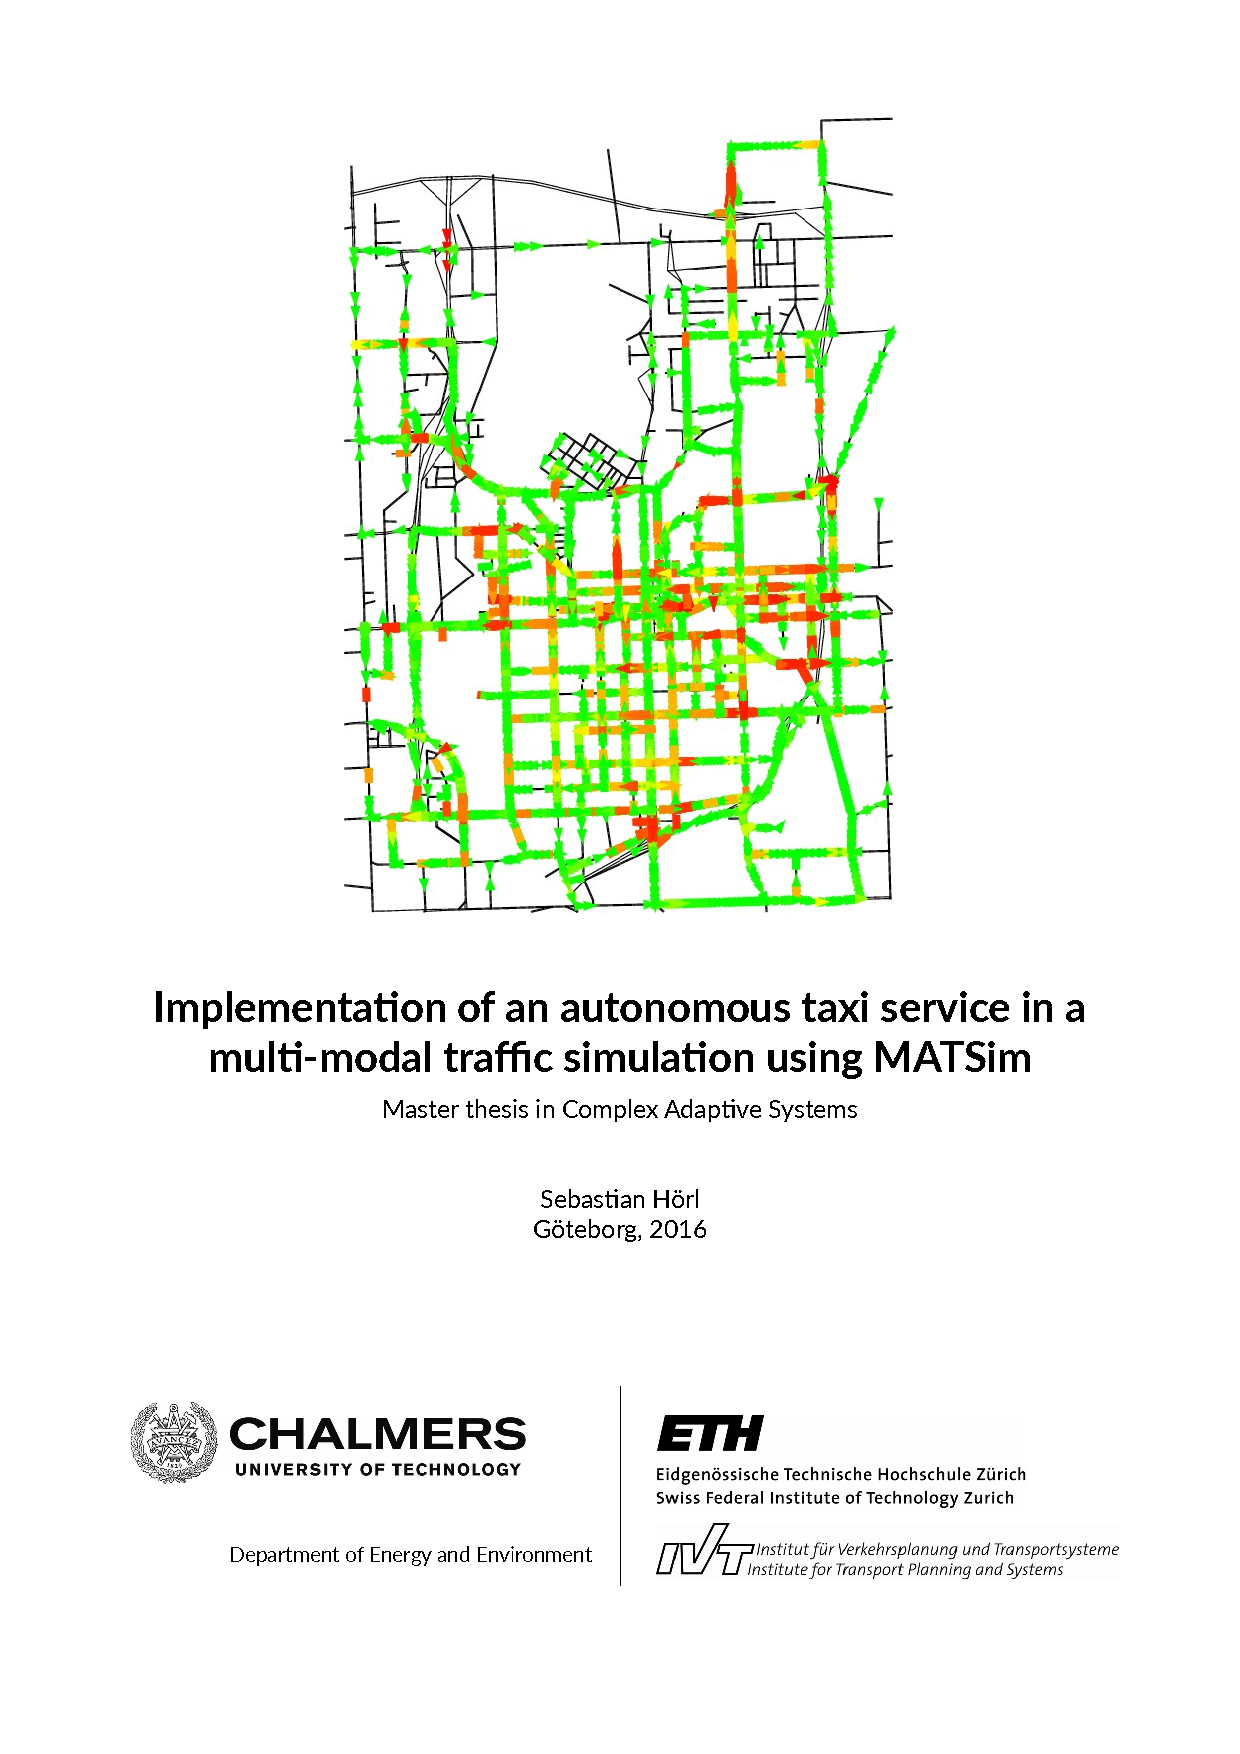
\includepdf[pages={1}]{cover.pdf}
\pagebreak

\pagenumbering{roman}

\tableofcontents
\pagebreak

\section*{Acknowledgements}
\pagebreak

\section*{Abstract}
\pagebreak

\section*{Kurzfassung}
\pagebreak

\section*{Abstrakt}
\pagebreak

\pagenumbering{arabic}

\section{Introduction}

Autonomous vehicles are expected to have a great impact on how the traffic situation
in our cities will look like in the not so far future. During the last years, autonomous
vehicle technology took great leaps forward, examples being Google's self-driving cars
\citep{Google2016} or Tesla's latest software updates on autonomous parking functionality \citep{Tesla2016}.
Furthermore, renowned car manufacturers such as Audi recently joined the competition.
Ambitious tests in real-world conditions are fostered all over the world, examples being Volvo's
DriveMe project with 100 autonomously driving cars on the highways of Gothenburg \citep{Gothenburg2016},
the LUTZ pathfinder project, establishing the use of three autonomous transport pods
in the city center of Milton Keynes \citep{MiltonKeynes2016} and a case study of
autonomous taxis in Singapore \citep{LTA2016}.

Especially big cities like Singapore could gain a lot from autonomous car technology,
be it from privately owned cars to publicly owned services. A floating fleet of
autonomous vehicles (AVs) could have a drastic impact on land usage, reducing the area of parking
space needed in the urban environment. At the same time, it has the potential improve road safety, access to transportation,
congestion, and emissions \citep{Kheong2014}. In fact, it is predicted
that an AV fleet size of one-third the size of the number of private cars could
serve the associated demand that is generated today \citep{Spieser2014}. From a user perspective, shared autonomous taxis could solve the classic ``last mile problem'' where AVs could
bridge the transport gap from the closest public transport facility to the homes
of the people \citep{Litman2014}. As soon as a particular supply of AVs is reached, prices are predicted
to become highly competitive to if not even cheaper than private car ownership \citep{Chen16}.

On the other side, with the adaptation of autonomous transport, fundamental moral
problems \citep{Hevelke2015a} need to be discussed, and related questions in liability and
ownership need to be answered \citep{Anderson2014a}. In general, predicting how and when autonomous
vehicles will be on the roads is a highly complex problem, and most of the proclaimed
benefits can easily be defeated due to a lack of reliable data.

To give an example, one of these benefits is having less congestion \citep{ITF2014}. However,
it is claimed that to make a passenger comfortable in a self-driving car,
significantly smaller accelerations and decelerations are allowed, and thus the
overall movements on the roads will be slowed down \citep{LeVine2015}. Therefore, having only assumptions
on how people would experience shared AV services, replacing a huge percentage of
contemporary cars with autonomous ones could in fact increase overall congestion.

Another example is the overall travel demand, which might increase with the introduction
of autonomous vehicles as a consequence of people seeing it as more convenient and
cost-efficient to other modes. This, in turn, could lead to the aversive effect
of increased congestion \citep{Litman2014}.

In consequence, while the technological development in autonomous driving already
came a long way, there is still much demand for research on an upper level, looking
at the overall economic and societal picture \citep{Silberg2013, SchoettleBrandon2014}. A valuable tool for doing this is the
use of traffic simulation \citep{Fagnant2014, ITF2014, Zachariah13}. Numerous efforts have been
made in predicting the usefulness of AVs for a city regarding AV supply, i.e.
answering the question how many shared AVs would be needed to serve an
existing demand fraction \citep{Bosch2015, Fagnant2015Austin}. On the contrary, fewer results are available on how the new travel
mode would interact with existing travel options and how customer preferences
influence the mode choice.

The agent- and activity-based traffic simulation framework MATSim \citep{Horni2015} allows for such
research \citep{Boesch2015} by taking into account assumed customer preferences and letting people
interact with a newly added means of transportation.
The framework has been successfully used in a range of studies from autonomous taxi services
in Berlin and Barcelona \citep{Bischoff2016} up to the simulation of the whole transport network of
Singapore \citep{Erath2014}. While the framework allows for a quite precise prediction of traffic
flows for scenarios involving car traffic and public transport, it yet does not
allow the simulation of dynamically acting autonomous vehicles embedded in the
overall traffic situation.

Therefore, the purpose of this thesis will be to implement means of simulating autonomous
taxis within the MATSim framework. Subsequently, measurements on how people would
switch to the new transport mode given certain supply levels, acceptance levels, and
pricing schemes will be made. A major challenge will be to account for an acceptable simulation
speed while keeping the dynamic detail, which is needed in order to simulate
intelligently acting AV taxi fleets. At the same time the functionality should be kept
as versatile and extendable as possible in order to make it possible to gain research
results on a multitude of factors, which influence the adaptation of autonomous
vehicles. Based on these criteria, a new framework for simulating dynamic agents
has been developed (\cref{sec:dynagent}).

In the scope of this thesis, a basic model of autonomous vehicles, which are transporting one passenger, is developed. Many
interesting aspects such as shared AVs, AVs for the purpose of feeding
public transport facilities or simulating a refuel/recharging infrastructure can
be subject of future research. Since the model relies on how likely
people are to use autonomous technology, the model at the moment will be mainly
pointed towards finding qualitative results on the interplay between factors that
define the traffic situation. However, customer preferences, actual experiences of AV technology and pricing information will
become available over the next years.

Given those data sets, the simulation developed in the thesis has the potential
to act as a valuable tool in transport planning and urban development. It will be useful
in planning for the implementation of the needed infrastructure, the development of
pinpointed transport solutions and a restructuring of the present traffic network
to account for the adaptation of autonomous vehicles.

The thesis at hand is structured in four main parts: \Cref{sec:matsim} will introduce how
traffic simulation is performed in the MATSim framework and highlight the aspects
that are important to know for the implementation of autonomous vehicles. \Cref{sec:sioux},
as another prerequisite for setting up a meaningful simulation, covers the adaptation
of the readily available MATSim scenario of the city of Sioux Falls. In \cref{sec:dynagent,sec:avmodel}, the technical implementation
of the AV simulation will be explained in detail on two abstraction layers, first
introducing a new framework for simulating dynamically acting agents in MATSim
and then creating a model of autonomous taxis based on that. Then, in \cref{sec:results}
the model will be tested with a variety of parameter configurations, giving
insights on the general working of the model and predictions of AV usage in the
artificial Sioux Falls test scenario. Finally,
\cref{sec:conclusion} provides an overview about the qualitative results, while
\cref{sec:outlook} will give an outlook on
a multitude of possible extensions of the model and further research questions that
can be answered using the model at hand.
 \FloatBarrier \pagebreak
\section{Simulation Framework}

The investigations of autonomous vehicles in this thesis will be based on the
agent-based transport simulation MATSim \citep{Horni2015}. The following sections
will outline how the framework works and where it can be extended to shape it
towards a autonomous taxi simulation. An overview will be given on which components
need to be modified and how the final transport situation will result from all
the different parts that are playing together in MATSim.

\subsection{Agent-based transport simulation}

The approach that is used in MATSim is to simulate a population on an per-agent
timestep-based level. At the beginning of a day each person in the synthetic
population has an initial plan of what it is supposed to do during the day. Mainly
those plans consist of two elements:

\begin{description}

\item[Activities] have a start and an end time, as well as, depending on the
respective scenario, certain constraints on when the earliest start or latest
end time could be. Alternatively activities could be defined using a certain
duration after which the agent needs leave the activity location. The ``standard'' activities are
``home'' (which usually is the first plan element of a day) and ``work''. More
elaborate simulations can additionally use an arbitrary number of secondary
activities.

\item[Legs] are the second type of plan elements. These describe connections
between two activity locations and contain information like which mode of transport
the agent will use (e.g. ``car'', ``public transport'', or ``walk'') and, depending
on the selected mode, further data like the route that should be taken through
the street network.

\end{description}

A typical day plan of a MATSim agent can be seen in \cref{fig:typical_plan}. The
agent starts at home, then walks to his job, stays there for a certain time and then
goes back home. Each agent in a poluation (which can range from several hundreds to
hundeds of thousands) has it's own individual plan that is executed when one day
is simulated.

\begin{figure}
    \centering
    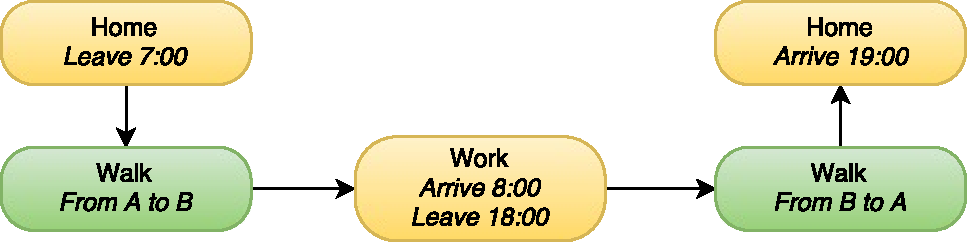
\includegraphics[width=0.8\textwidth]{figures/simpleplan.pdf}
    \caption{A typical agent plan in MATSim}
    \label{fig:typical_plan}
\end{figure}

The network, on which the simulation is taking place, is decribed through nodes
 and connecting links. These are described by a specific capacity which tells the
 simulation how many vehicles are able to pass the link within a certain time
 frame, while the the length and an average link speed determine how fast vehicles
 will travel to the next node.

 The whole MATSim simulation is done time-step by time-step. In a single simulation step (usually 1 second)
 the agents that are currently in an activity don't need to be taken into account unless their scheduled
 activity end is reached. The other agents, which are currently on a leg, are simulated in a
 dedicated traffic network simulation. This simulation moves the agents according
 to the capacity and current congestion from the start node to the end node of the
 respective links. Traffic is not simulated on a micro-level (i.e. the vehicles
 don't have distinct positions along the link) in order to increase the simulation
 speed.

The congestion on the traffic network is therefore emerging from the single travel
plans of all the agents. If there are too many agents which try to use one route
at the same time, the overall congestion will increase.

All steps described above, i.e. the simulation of acitivities and legs during
a whole day, are summarized as the ``Mobility Simulation'' or, in short, Mobsim
of the MATSim framework.

In order to simulate dynamic agents, which are not statically residing in a
fixed-timed activity or a predefined leg route, quite significant changes need
to be made and some of the computational advantages of the simulation approach
need to be partly circumvented. This, however, mainly addresses implementational
details and will be discussed later throughout the thesis in \cref{sec:dynagent}.

\subsection{Utility-based scoring}

As pointed out in the last section, individual travel decisions might lead to
waiting times on the network, which then can also lead to late arrivals at the
designated activity locations, which usually would be disadvantageous in the real
world. Therefore, it might be beneficial for an agent to reconsider the time and
route choices that had been made for the current day, just as a real person
would do.

In order to ``know'' whether a plan worked out well or was disadvantageous, the
single elements need to be weighed and quantified. This is done using the Charypar-Nagel
scoring function \citep{Horni2015}:
\begin{equation}
S_{plan} = \sum_{q=0}^{N-1} S_{act,q} + \sum_{q=0}^{N-1} S_{trav,mode(q)}
\end{equation}

Basically, it combines the marginal utilities of all activities ($S_{act,q}$) ranging
over the $N$ activities in a plan and the marginal utilities for all the legs in
between.

The marginal utility for the activities, among other factors, depends on how long
the activity has been performed, whether the agent needed to wait to start it (due
to an early arrival) or whether it was forced to leave early. For more details
the complete computation is shown in \citep{Horni2015}.

For the scope of this thesis the travel utility is more interesting. A basic version
for a single leg $q$ can look as follows:
\begin{equation}\begin{aligned}
S_{trav,mode(q)} = C_{mode(q)} + \beta_{trav,mode(q)} \cdot t_{trav,q} + \gamma_{d,mode(q)} \cdot \beta_{m} \cdot d_{trav,q}
\end{aligned}\end{equation}

\begin{description}

\item[Mode Choice] The first term, $C_{mode(q)}$, describes a constant (dis)utility for the
choosing a certain mode for the leg. It can be interpreted as how ``favorable''
a certain mode is and is generally negative.

\item[Travel Time] The parameter $\beta_{trav,mode(q)}$ is the marginal utility of traveling,
which is multiplied by the time spent on the leg $t_{trav,q}$. It signifies how
favorable it is to spend time on such a leg, i.e. the longest one needs to stay
in a car or in the public transport, the larger the disutility gets (and therefore
the parameter is usually negative). Values which are absolutely bigger therefore
stand for travel modes where time is spent less useful or comfortably.

\item[Travel Cost] The third element involves the (positive) marginal utility of money $\beta_{m}$,
which is an universal simulation parameter and describes how the utility of money can
be weighed against e.g. time.
It is multiplied with the (negative) monetary distance rate
$\gamma_{d,mode(q)}$, which states, to how much disutility per spanned
distance the leg will lead. This parameter is useful for imposing distance-based
fares in a certain transport mode and thus making it monetarily attractive or
unattractive compared to other ways of traveling.

\end{description}

Beyond these parameters, which are usually used by all travel modes, there are
a number of additions, e.g. for public transport, or yet generally unused options, such
as a direct marginal utility of distance travelled.

For the purpose of simulation autonomous taxi services, two additions are made:
\begin{equation}\begin{aligned}
S_{av} &= C + \beta_{trav} \cdot t_{trav} + \gamma_d \cdot \beta_m \cdot d_{trav} + \beta_{wait} \cdot t_{wait} + f_m(d_{trav},t_{trav})
\end{aligned}\end{equation}

\begin{description}

\item[Waiting Time] Here, $\beta_{wait}$ is the marginal utility of waiting time, quantifying
how disadvantageous it is to wait for a taxi to arrive.

\item[Service Cost] Furthermore the function
$f_m(\cdot)$ is a placeholder for any pricing strategy that might be tested (on top or as a replacement for the beforementioned travel cost). The
implementation will allow for an easy modification of this function.

\end{description}

\todo{Explain double penalty for waiting time due to less time to do activities}

All these utility computations are done after all agents have been simulated for
a whole day (in fact, usually 30h are used). This step in the MATSim framework is
simply called the ``scoring'' phase.

\todo{It would be better to explain the additional parameters further down
in the chapter about the AV fleet model. Here, further explanations on how those parameters
are usually measured and estimated would be more adequate.}

\subsection{Evolutionary replanning}

The last step in order to make all the agents ``learn'' more optimal plans which
make sure that they arrive on time at the activity locations and avoid congestion
is to make them replan their day. This is done using an evolutionary algorithm in
the following way:

Usually an agent will start out with one quite random plan, go through it during
one whole day and then get a score for it. Afterwards, in some iterations, this
plan is copied and modified slightly. Those modifications can happen with respect
to start and end times of activities, mode choices for certain legs, etc. So after
one iteration the agent might already have two plans to choose from.

Before the next day starts, one of the available plans is selected due to a certain
strategy. The standard approach is to do a multinomial selection with respect to
the previously obtained plan scores. So one after another plans, will be created,
scored, modified, rescored and so on. Because of the selection process, which
favors high scores, better and better choices will be made.

However, this is done for each and every agent, so while improving the performance
of one agent's plans, this might effect the performance of other agents negatively,
which is especially true if one thinks about the example of highly congested roads
due to too many agents choosing the same route. Finally though, the algorithm reach
at a quasi-equilibirum, which in MATSim is usually refered to as the ``relaxed
state'', in which the average score of the used plans stabilizes within a
reasonable variance.

Each ``day'' that is simulated in this manner is usually called an ``iteration''
of the simulation. It is common to divide these iterations into two parts. The
first one is the ``innovation phase'', where plans have a certain probability to
be modified, while in the second phase innovation is turned off. This means that
the agent will only choose among the present plans in his repertoire (usually
around 5) and rescore them again and again, until the most favorable is selected.

All of the above is known as the ``replanning'' in MATSim. Putting everything
together, a whole cycle in a MATSim simulation can be seen in \cref{fig:matsimcycle}. Since the
final traffic situation evolves from the evolutionary choice in the replaning and
selection, as well as from the emergent congestion in the Mobsim, this whole
cycle is usually referred to as a ``co-evolutionary'' algorithm.

\Cref{fig:scorestats} shows a typical progression of the population-wide score in
a MATSim simulation. What one can see there is an average over the worstor best plans
of each agent, additionally the averaged average score of all the plans that the agents
own is displayed. Finally one can see the average of all the plans that have been executed
by the agents in a particular iteration.

The first phase until iteration 100 is the innovation phase, where time and mode
choices can be done, while at iteration 100 it is turned off. There, because now
the best plans must adapt to the overall situation, they are loosing in value,
while the worst scored plans are dropped are likely to be discarded. Finally,
a quite stable population-wide relaxed state is reached.

\begin{figure}
    \centering
    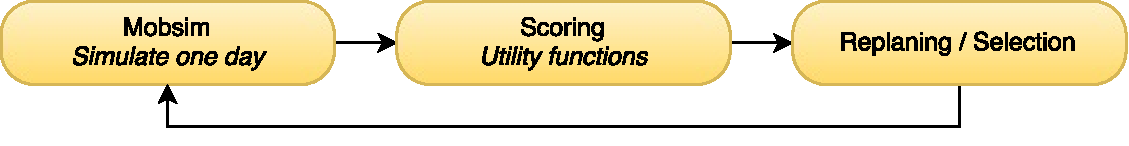
\includegraphics[width=1.0\textwidth]{figures/matsimcycle.pdf}
    \caption{The basic co-evolutionary algorithm of MATSim, showing the three main
    stages: Mobsim, Scoring and Replanning/Selection}
    \label{fig:matsimcycle}
\end{figure}

\begin{figure}
    \centering
    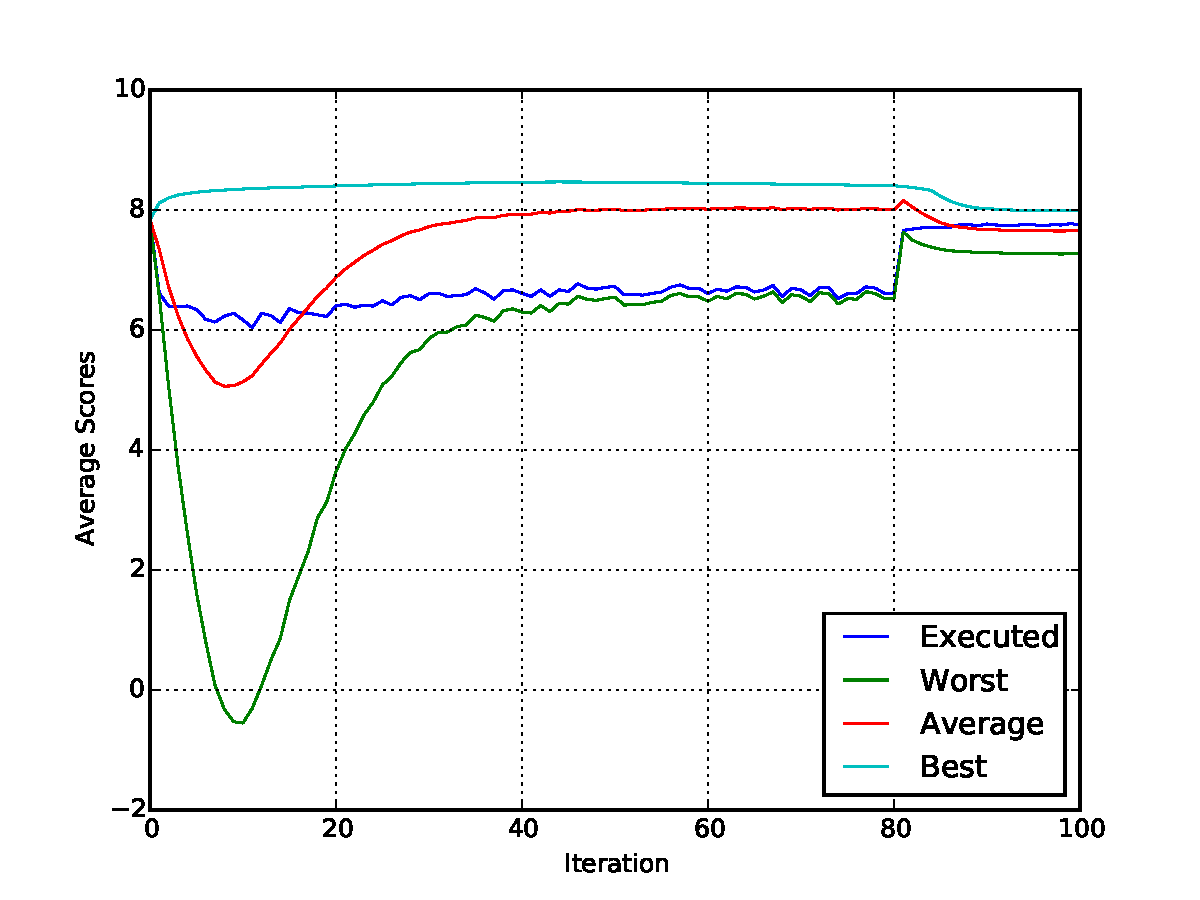
\includegraphics[width=1.0\textwidth]{figures/scorestats.pdf}
    \caption{Typical progression of the agent scores throughout a MATSim simulation.
    ``Worst'' means that the plans with the worst scores from all the agents are taken
    and averaged, the same applies for the other graphs. \todo{make a better graphic with a more clearer relaxation (simple corridor should be okay)}}
    \label{fig:scorestats}
\end{figure}

\subsection{Queue-based simulation}

The heart of the simulation in MATSim is the queue simulation, or more briefly,
the QSim. This part of the framework is iterating through all the agents that need
to take action in the current simulation step.

Itself the QSim is split into the handling of agents which are currently performing
an activity (i.e. are in an idle state in terms of the traffic simulation) and another
part, the Netsim, which is simulating the traffic network.

When running the Netsim, the agents are moved on the network according to their
current route and dependent on congestion. After moving an agent, the Netsim checks
whether the agent should end its trip at the current link he has been moved to. If
this is the case, the agent is removed from the Netsim and the next agent state is computed.

The result of this computation is either that the agents wants to start a leg, in
which case he is reinserted into the Netsim, or that he wants to start an activity,
which will make the agent to be added to the activity queue.

This activity queue is the other main component of the QSim. In fact it is a
priority queue, where all agents are sorted according to the time at which they
want to end the next actvity. So when adding an agent to the activity queue it first
is checked when the activity should be ended and then the agent is inserted at the
corresponding position in the queue.

The processing of this queue in the QSim for each simulation step then works as
follows: The first element of the queue is looked at and it is checked, whether the
agent should already end the activity. If this is not the case, the simulation step
is already finished. On the other hand, if the activity should be ended now (or
previously if the time resolution of the simulation is quite high), the agent is
removed from the top of the queue and the next state is computed as described above.
Then the new top element of the queue is examined, until the simulation step is
finished. The whole QSim simulation is schematically rendered in \cref{fig:qsim}.

The big advantage of this simulation architecture is as follows: When an agent is
in an activity, no computation needs to be performed. So instead of polling all
the agents in every simulation step to check if they want to end an acitivity, the
computational demand is much lower when using the queue, since a lot of agents can
be skipped. The sequential processing of the priority queue is very fast in terms
of computational complexity ($\mathcal{O}(1)$ for checking the top element
and $\mathcal{O}(\log n)$ for fetching it, \citet{JavaPQ})

Furthermore the same concept is used within the Netsim to speed up the computation
of the traffic situation. In both cases, for the QSim and Netsim, those savings in
computation time naturally decrease the versatiliy of the simulation environment.

One major drawback is that if an agent, which is already queued should abort its
current activity, it needs to be removed from the queue and added at a new position.
Both operations are quite costly for the priority queue \citep{JavaPQ}, so
if more and more reschedulings are needed, the computational overhead can become
quite large.

However, for truly dynamic agents, like autonomous vehicles, it is necessary to
adopt their plans frequently and thus some thought needs to be put into how to
achieve this freedom while still keeping as many advantages from the existing
simulation architecture.

\begin{figure}
    \centering
    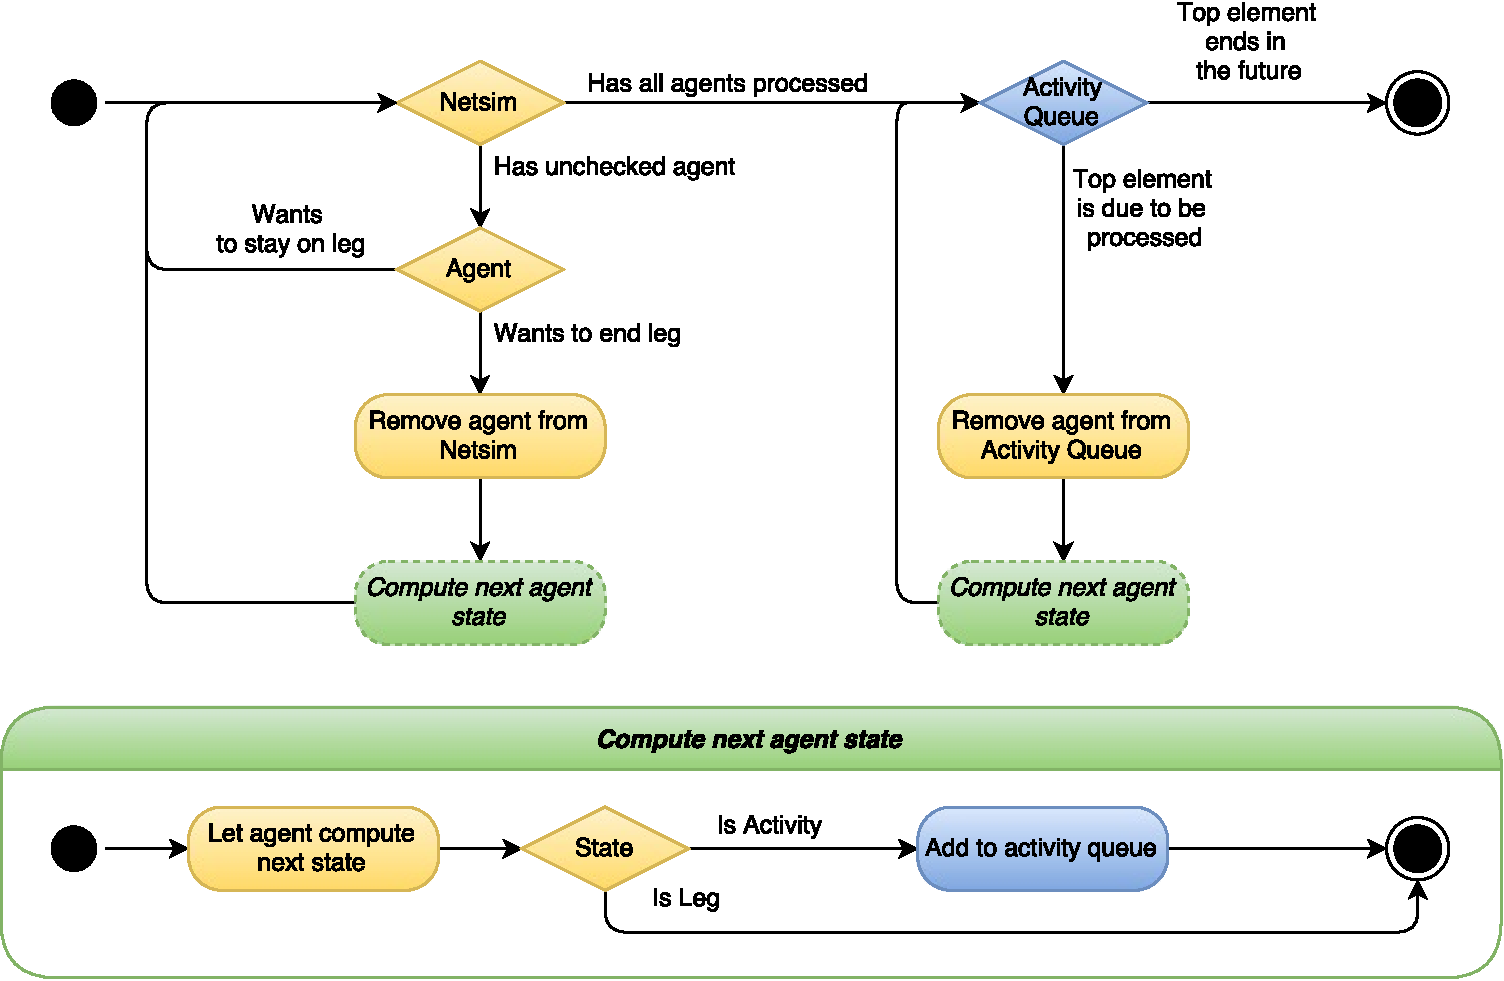
\includegraphics[width=1.0\textwidth]{figures/qsim.pdf}
    \caption{Simplified structure of the QSim in MATSim.}
    \label{fig:qsim}
\end{figure}
 \FloatBarrier \pagebreak
\section{The Sioux Falls Scenario}
\label{sec:sioux}

The City of Sioux Falls in South Dakota (\cref{fig:original_map}) has been a classic test case in transport
research for more than four decades, being first mentioned in this context in
\citet{Morlok1973}. While none of the numerous implementations of the network are intended to be accurate
and realistic with respect to the actual City of Sioux Falls, they are merely aiming
towards providing downscaled, computationally tractable test cases for transport
planning and simulation problems.

In \citet{Chakirov2014}, the scenario (``Sioux-14'', \cref{fig:sioux14}) has been
adapted to the MATSim framework. A sparse street network, which is computationally
easy to handle by the simulation, was introduced. It consists of 27 nodes and 76 links,
representing the main arterial roads of the city, split further down into
282 nodes and 334 links in order to arrive at partial link sizes of less than $500m$.
This is necessary because MATSim agents start their travels at the start node
of a link and thus a high resolution is needed to avoid unrealistic clustering.

\begin{figure}
    \centering
    %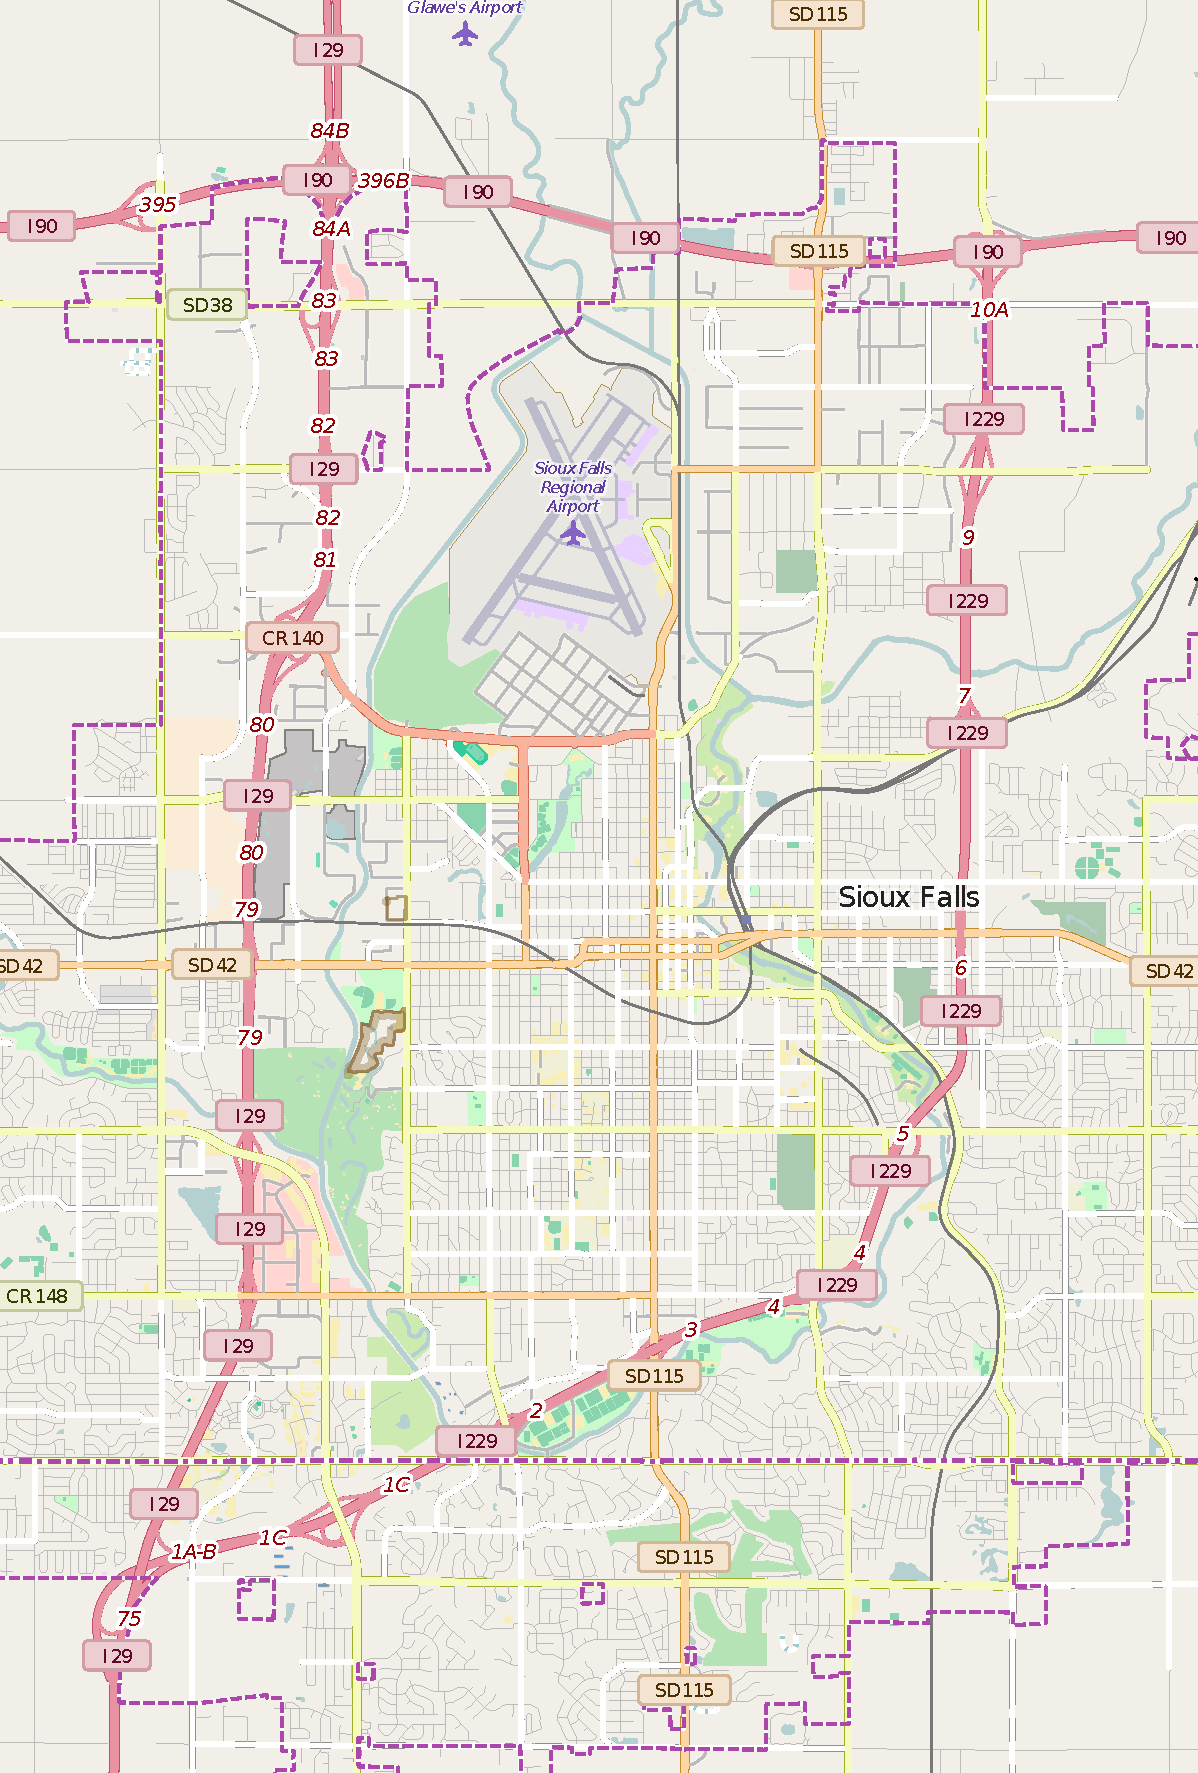
\includegraphics[width=0.8\textwidth]{figures/original_map.pdf}
    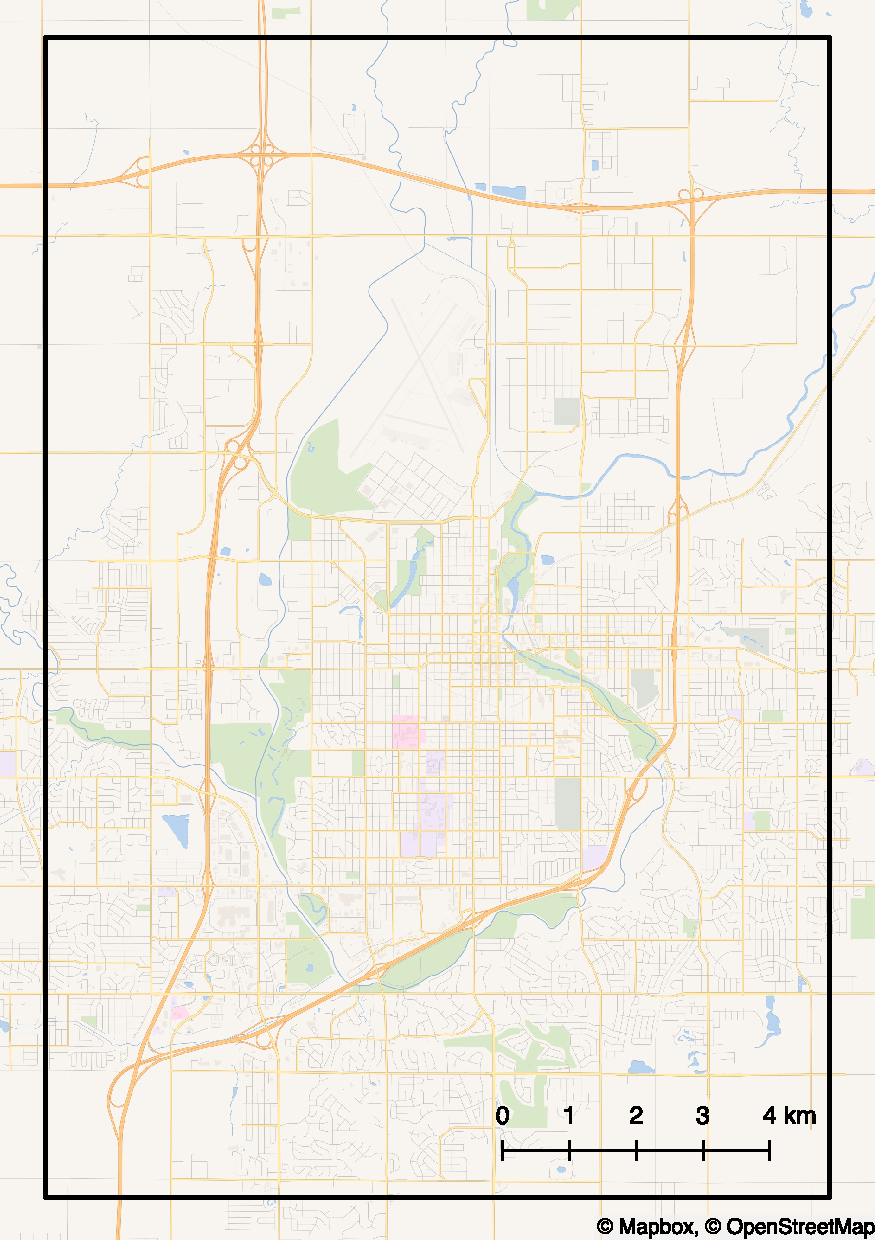
\includegraphics[width=1.0\textwidth]{figures/sioux_falls.pdf}
    \caption{Map of Sioux Falls. The bounding box encapsulates the
    processed region with longitude from $-96.8105°$ to $-96.6653°$ and latitude from $43.4729°$ to $43.6286°$.}
    \label{fig:original_map}
\end{figure}

\begin{figure}
    \centering
    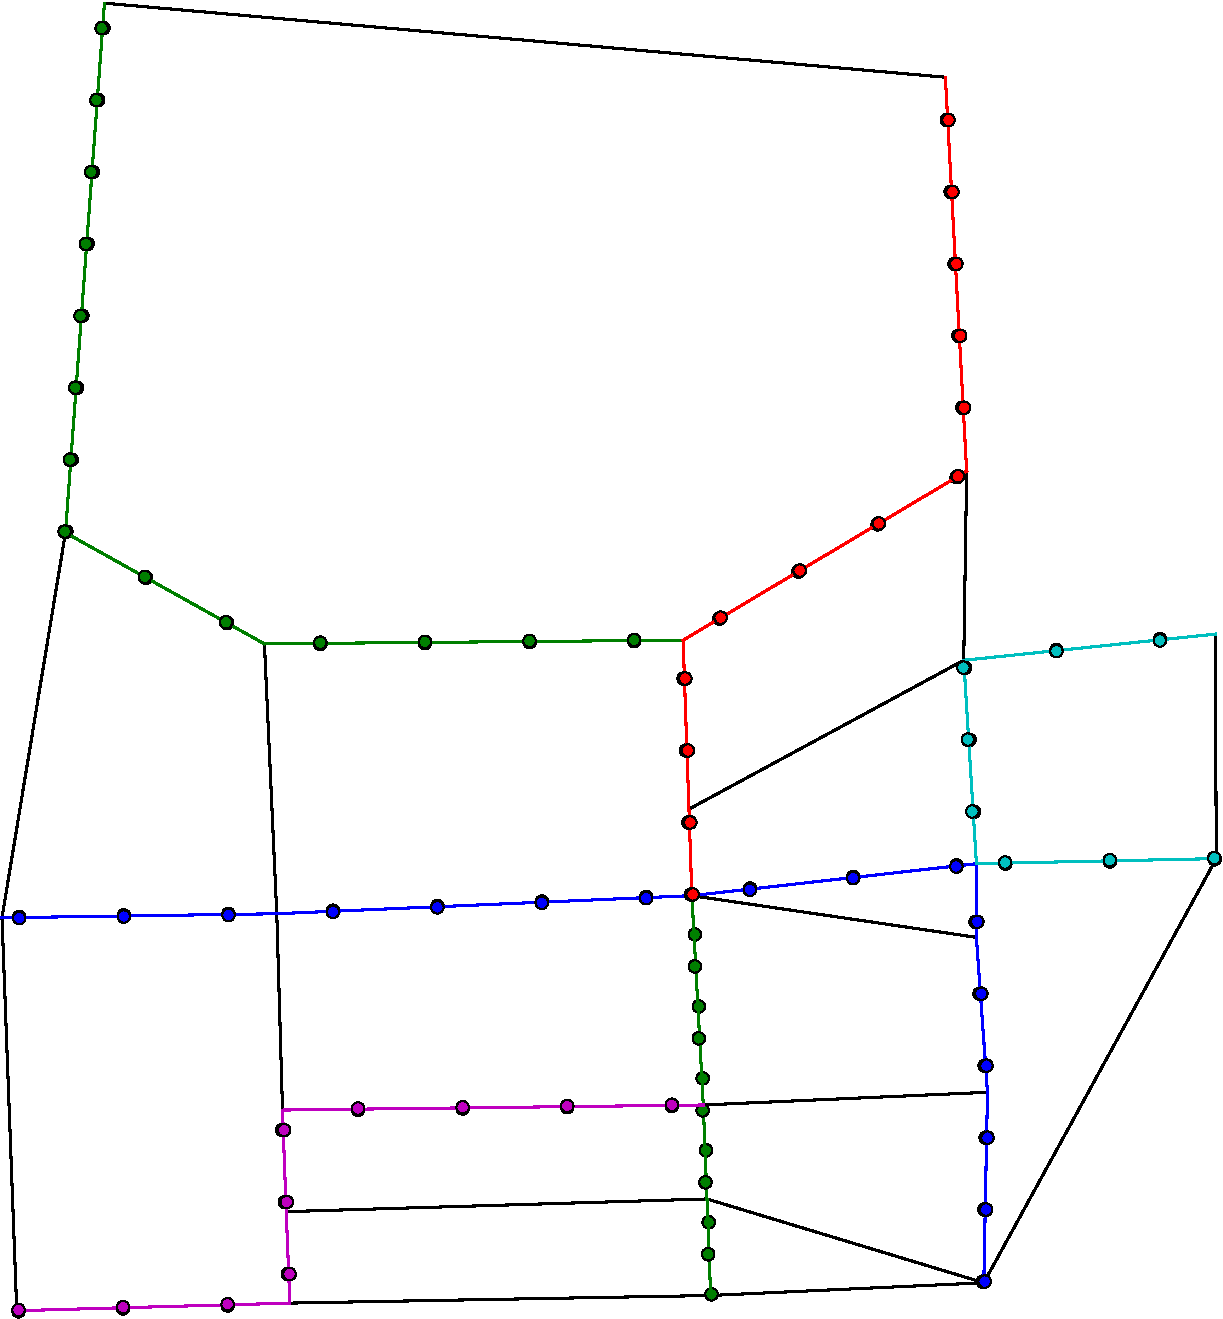
\includegraphics[width=0.4\textwidth]{figures/sioux14_pt_cropped.pdf}
    \caption{Sioux-14 road and public transport network}
    \label{fig:sioux14}
\end{figure}

On the supply side, there is furthermore a public transport network, which
consists of 5 lines with bus stops along the arterial roads in a distance of $600m$.
The stops are placed at a distance of $5m$ perpendicular to the road and departures
from the lines' respective start links take place every 5 minutes.

Much of effort has been put into the modeling of the demand side, covering the
realistic generation of home locations, workplaces, secondary activity locations,
as well as the distribution of socio-economic factors such as age, car ownership
and gender across a synthetic population, as it is needed for the agent-based
simulation.

In this regard, the scenario provides a lightweight example of a complete MATSim
simulation, where it is easy to test different parameters and extensions to the
framework on a near-realistic baseline scenario. However, while working with the
original Sioux-14 network during the course of this thesis, it became evident that
the simplified structure of the underlying traffic network does not provide enough
resolution for the simulation of autonomous vehicles.

The main reason is that agents, who choose to take a car in the Sioux-14 network,
probably living in the middle of the rectangular regions of the network would be
teleported to the nearest link to start their travels. This would also be true
for autonomous vehicles, which is not a realistic assumption in both cases, especially
when comparing it with public transport, where agents in MATSim are explicitly
penalized for covering the distance between home and bus stop by foot.
Furthermore, the effect of people being more inclined to opt for an autonomous taxi
when living far from public transport can only be convincingly simulated on a
finer network.

The following sections will describe how, starting from the initial Sioux-14
scenario, a new more fine-grained versatile test scenario for MATSim has been
developed, which in turn has been used as the basis of the following investigations in this
thesis.

The new Sioux-16 network, which has been developed in this thesis, is based on the
demand model of Sioux-14, which means that all locations for homes, workplaces and
secondary activities are kept equal, while it differs on the supply side, aiming
to resemble the original scenario as closely as possible. The following sections
will describe, how the Sioux Falls network from OpenStreetMap (with the state
as of 18 Apr 2016) has been converted and adjusted to be compatible with MATSim
and closely match the prior version of the test scenario. Furthermore, it will
be explained, how the public transport network has been adapted to the fine-grained
Sioux-16 scenario.

\subsection{Network generation and adjustment}

For the creation of the new scenario, an area covering Sioux Falls has been captured
from OpenStreetMap, which can be seen in \cref{fig:original_map}. Using the MATSim
exporter in the JOSM tool \footnote{https://josm.openstreetmap.de/}, a simplified,
MATSim-compatible network of the selected region has been created. In this process,
all primary, secondary and tertiary streets have been selected, while road types
further down the hierarchy (for instance residential streets) have been omitted.

However, some adjustment was needed for the network to play nicely with
the given facilities from the Sioux-14 scenario. Most importantly, the network from
OSM was defined in the EPSG:3857 coordinate system, while Sioux-14 uses EPSG:26914.
Therefore, in a first step, the coordinates of all the generated nodes needed to
be converted to the old system.

In a second step, the positions of all facilities in Sioux-14 have been obtained
and a bounding box with a margin of $500m$ around them has been computed. Subsequently,
all links, which were located out of the bounding box, were removed from the network,
while those who were crossing the borders have been cut to fit into the area. The
initial network with all removed (red) and cut (blue) roads can be seen in \cref{fig:sioux_step2}.
In total 352 outside links have been removed, and 83 links have been adjusted.

\begin{figure}
    \centering
    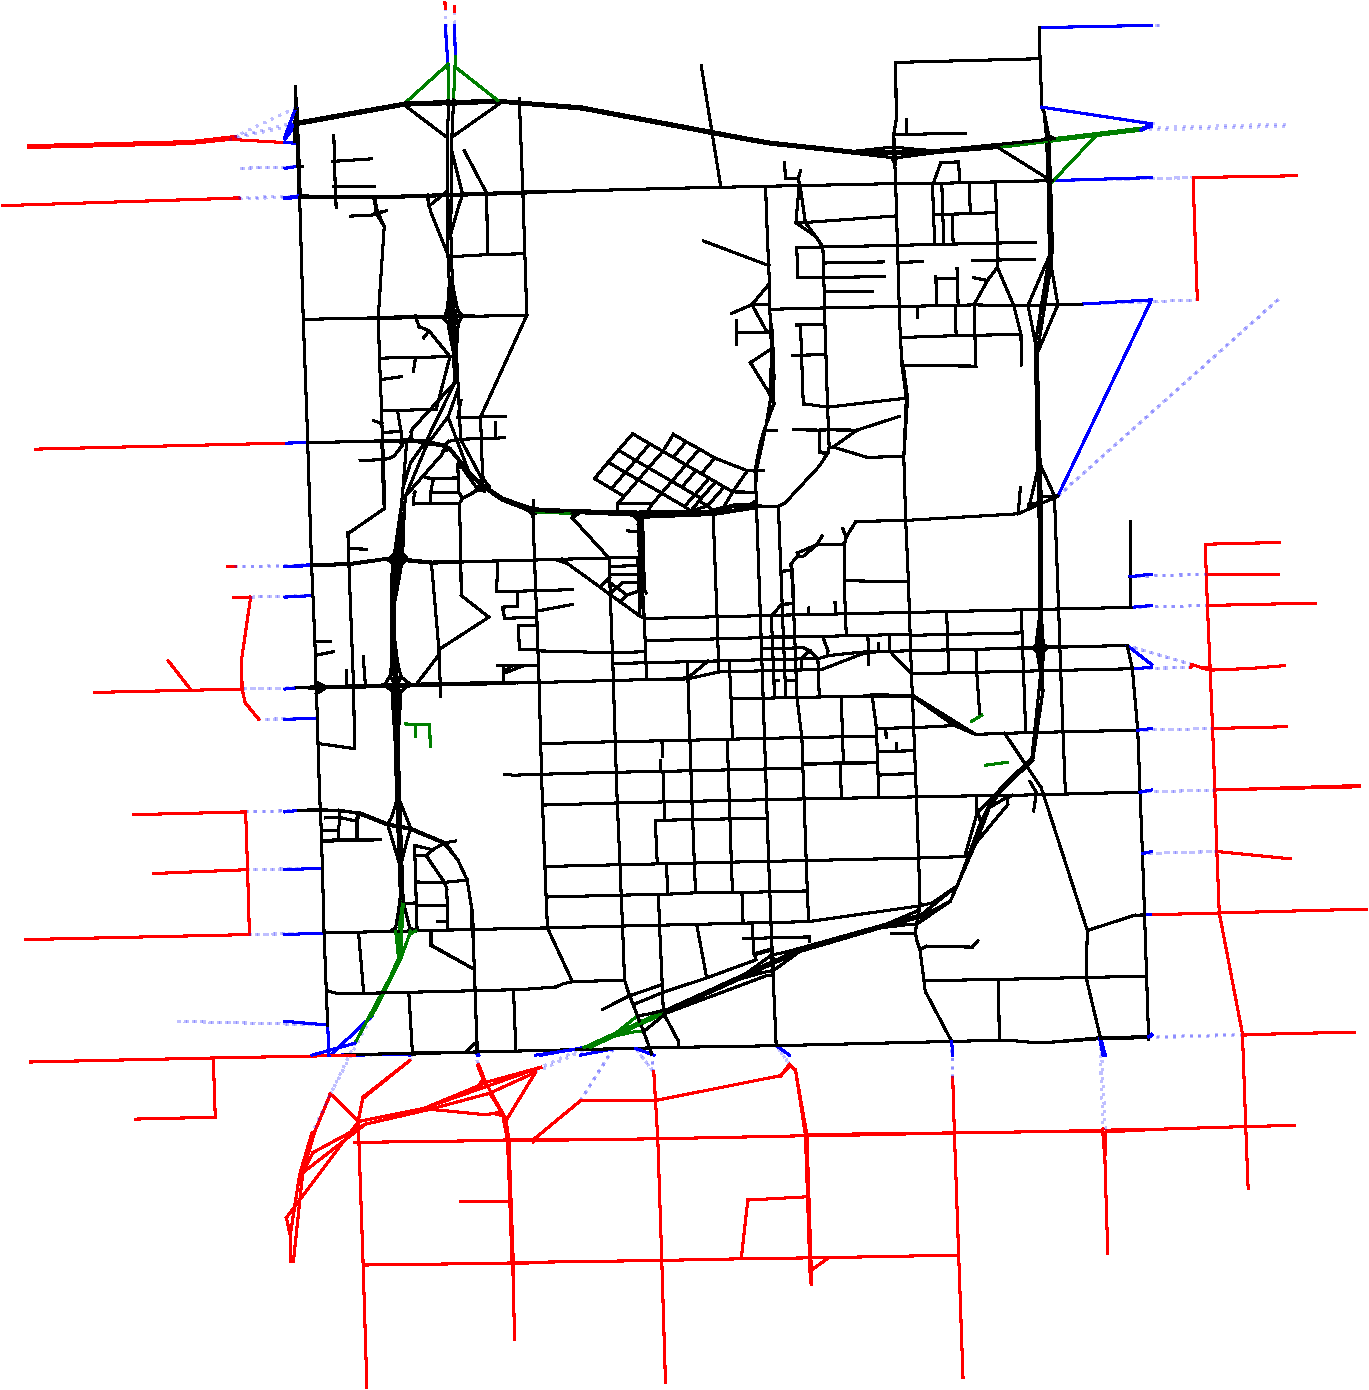
\includegraphics[width=0.6\textwidth]{figures/sioux_step2_cropped.pdf}
    \caption{Automatic network modifications: Red links have been removed while
    blue links have been shrunk to the closest border points of a bounding box
    enclosing the facilities of the scenario. Green lines have been removed either
    for being detached from the main network being sinks/sources.}
    \label{fig:sioux_step2}
\end{figure}

After that, a cleanup up the network needed to be done, partly because of artifacts
due to the filtering of road types, partly because of the removal of the external
sections. This removal was done in a couple of steps:

\begin{enumerate}
\item The lengths of all the links have been updated to the $L^2$ distance of their
respective start and end nodes in the new coordinate system.
\item The network has been searched for sources (nodes that only have outgoing links)
and sinks (nodes that only have incoming links). Those have been removed, because they
make no practical sense. This proecdure lead to 53 removed links in total.
\item One seed node has been defined, which definitely belongs to to the street
network and then by traversing the all paths from that node, it has been determined,
which streets belong to the main network. All remaining nodes and links, which have
become detached from this main network have been removed (11 nodes and 14 links).
\item Finally, the network has been searched for duplicate links with the exact
same start and end node. Only the first of those links have been kept, which lead
to the removal of 3 duplicates.
\item In Sioux-14, the links have been split such that there are no connections
longer than $500m$. This procedure has also been applied to the network at hand,
leading to 389 split links, which have been cut into a number of equal parts
with less than $500m$ length depending on their overall length.
\end{enumerate}

Regarding nodes, these procedures in total lead to an increase of nodes from
$1392$ to $1806$ and in an increase of links from $2957$ to $3335$. The links
that have been removed during the cleanup are colored in green in \cref{fig:sioux_step2}.

\subsection{Public Transport Adaptation}

The adaptation of the public transport network to the new (``Sioux-16'') scenario posed some
challenges that needed to be solved:

\begin{itemize}
\item The links of the original network did not exist anymore, obviously the
routes for the different public transport needed to be mapped to the new network.
\item The stops from the original network could not be mapped easily to the new
roads, partly because some streets in Sioux-14 were ``invented'', only approximating
connections in the finer network on a very coarse level, but also because roads
that consisted of two overimposed links for both directions were now split up into
two spatially distinct lanes (as can be seen in the upper left part of \cref{fig:pt_network}).
\end{itemize}

In order to get a rough routing for the bus lines, the main nodes of the Sioux-14
network have manually been mapped by hand to nodes in the Sioux-16 network. This
made it possible to obtain new public transport roads in terms of those guide points:
For each of the lines it has been defined, which guide points should be traversed
and in which order. Then, the Dijkstra algorithm \citep{Dijkstra} with travel time as the objective
has been used to find the shortest path from waypoint to waypoint. After fitting
those partial paths together, the whole routes in terms of the links of the Sioux-16
network have been obtained. As can be seen in the colored routes in \cref{fig:pt_network}
this made it easy to obtain routes that take into account the specific map structure
(for instance the highway on the upper left or the one-way streets, which are
traversed by the blue line in the center of the map).

The generation of bus stop facilities was a more challenging problem. Given the
location from Sioux-14, one could roughly match the stops to links along the new
routes, which worked in principle. However, using this approach, bus stops were
cluttered all along the lines. With the intention of having a rather realistic
network some conditions needed to be taken into account:

\begin{itemize}
\item The bus stops of one line should be on opposite sides of a street and not
have a large longitudial distance. While satisfiying results could obtained, for
instance in the center with the blue line, the same approaches did not work well
for the highway connectors on the left for the green line, and vice versa.
\item The bus stops of parallel lines should be at the same locations, i.e. in
the center where the green line uses the same roads as the red one, the same
locations should be chosen. This constraint usually interfered with the approaches
that took into account the first constraint (especially in the center for the
blue line).
\item Finally, some of the Sioux-14 locations where completely off the network in Sioux-16,
for instance for the red line, where one can see a bend in the diagonal connection,
which was modelled as a straight line in Sioux-14.
\end{itemize}

Given all those constraints the best approach seemed to put in manual work with
some automated help. The final approach made use of a small program, written to
manually choose the stop locations along all roads and then subsequently choose
which stop locations should belong to which line. In this step one did not take
into account the cases of two lanes, as just the general positions needed to be
known (e.g. for the blue line in the center an approximate position between the
two lines would be chosen).

In another step, the locations that had been assigned to each line have been
assigned to the respective links along the line. So for the blue one, the average
points in between would have been assigned to a link underneath for one direction,
and another stop would be created for the link above. This resulted in a final
set of stop locations.

Furthermore, some stop locations were located on one single link. This
can happen if there is a link of roughly $500m$ and the stops are for instance
located at $1m$ and $499m$ along the link. In those cases, the network needed to
be broken up at those positions. In the current scenario, this leads to the splitting
of only four links.

Finally, according to the setup of Sioux-14 the stop locations have been moved
to a position normal to the link direction, with a distance of $5m$. Additionally
a schedule with buses departing in $5min$ intervals has been created.

The final public transport network can be seen in \cref{fig:pt_network}. It features
150 stops with an average distance of $520m$ and a median of $566m$. This is a
result of not being able to put the stops as accurately in intervals of $600m$
as it is possible in Sioux-14. Moreover, the $L^2$ distance between two stops along
the routes have been used instead of a measure along the actual path. The minimum
and maximum distance between stops are $218m$ and $847m$, respectively.

All steps that have been described above have been implemented in a reusable and
parametrized way. For instance, one could choose to allow a maximum link length of
$5km$ and would still obtain a valid network at the end, probably just with a larger
number of split links during the processing of the public transport.

\begin{figure}[h]
    \centering
    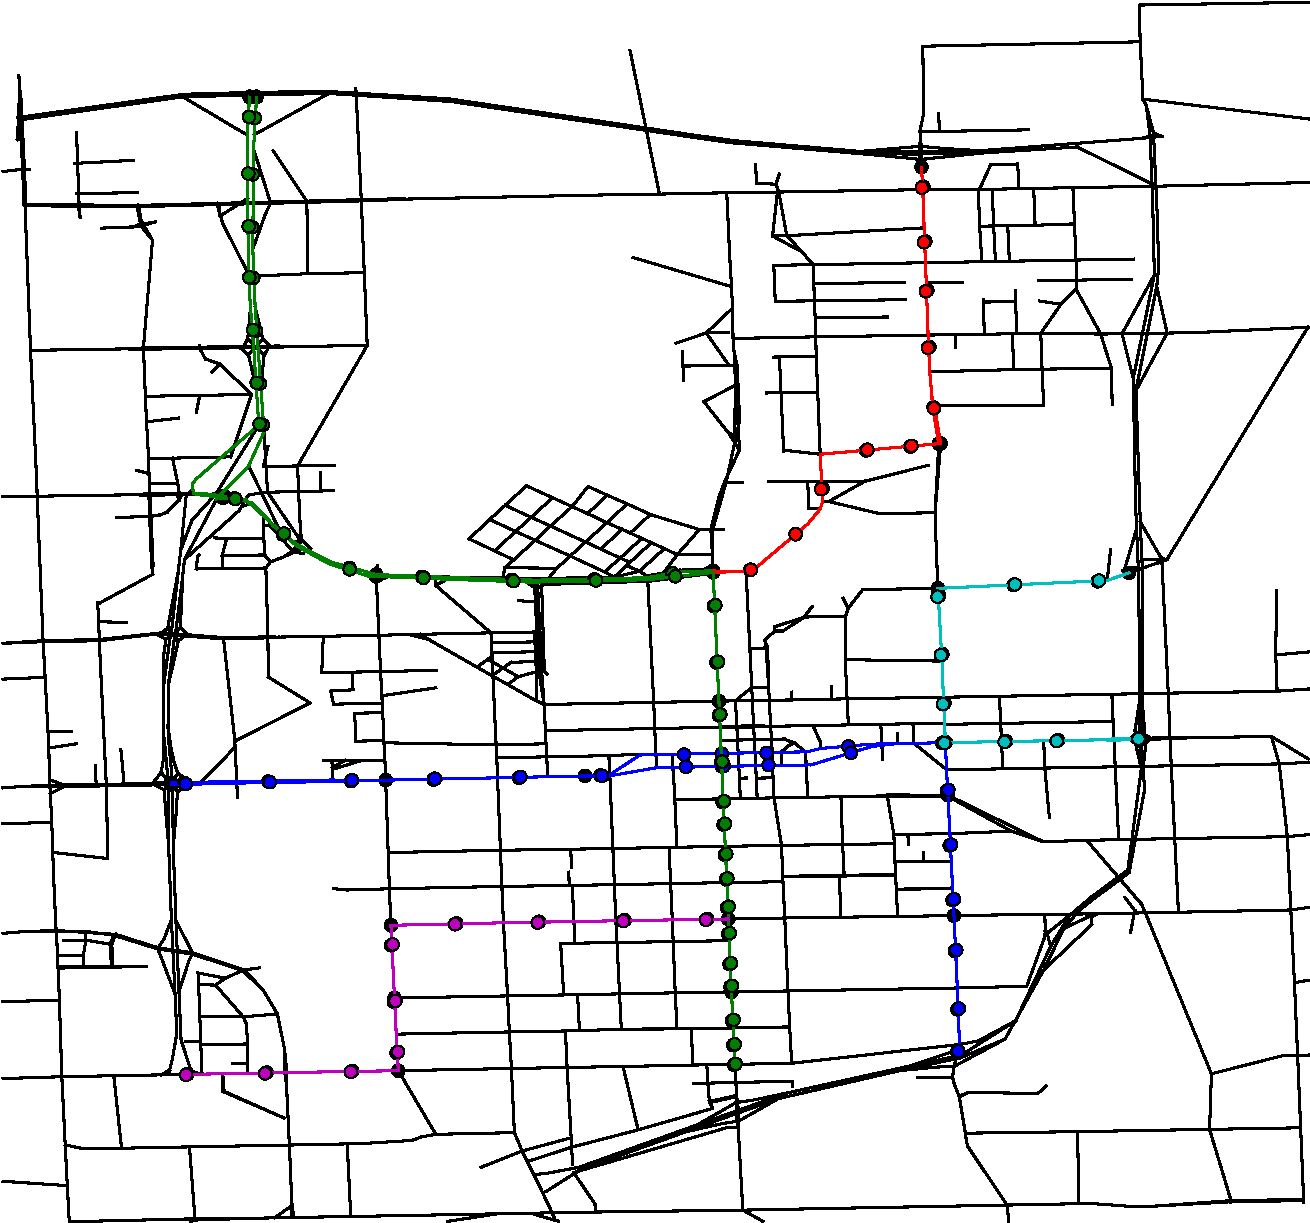
\includegraphics[width=0.8\textwidth]{figures/pt_network_cropped.pdf}
    \caption{Sioux-16 network with five public transport lines and respective stop
    facilities}
    \label{fig:pt_network}
\end{figure}

\subsection{Scenario Calibration}

The Sioux-14 network features artificially chosen link capacities, which are based
on a minimum of two and a maximum of three lanes per link, where three have only
be chosen for a fraction of highway links \citep{Chakirov2014}. While the added
minor streets in Sioux-16 should not make too much of an impact on overall
capacity, the highways and main arterials of the real network usually feature
greater capacity (for instance by providing \textit{four} lanes on the western highway).

Looking at \cref{fig:sioux_times}, it can be seen that the travel time (of cars) in
the new network is lower (red), compared to Sioux-16 (black). This effect can partly
be explained by the increased capacity, but also by the multitude of new options
to choose the most effective route for a trip through the fine-grained network. In
fact, the route choice might be the major influence when comparing with the data
from \cref{fig:sioux_speeds}. There the decrease in link speeds (relative to the freespeed) can be seen, which
is quite similar, indicating a comparable amount of congestion in the network.

Depending on how important the comparability to Sioux-14 in a specific scenario
is and what time of the day should be compared, it might be beneficial to adjust
the flow capacity of the network\footnote{In MATSim, this can be easily done
in the Mobsim configuration, e.g. \texttt{qsim.flowCapacityFactor} for QSim}:
In terms of travel times a scaling of 50\% would resemble the afternoon peak
way better than the 100\% version, while the morning peak would best be recovered
by a value in between (\cref{fig:sioux_times}). A similar situation arises for the
link speeds in \cref{fig:sioux_speeds}, where a value of 50\% is better suited for
comparing the morning peak while the 100\% scaling creates more comparable
results in the evening.

Furthermore, in terms of link speeds, it can be seen that the Sioux-16 scenario
features less congestion during the off-peak hours due to the possibility of
distributing trips all over the network.

In any case it has to be kept in mind that comparing the speed decreases is only
a rough measure of network congestion. Most importantly, the values displayed are
average values, which means that they biased towards outliers, i.e. capturing the
changes in main arterials. That is a good comparison to Sioux-14, but on the other
hand, the average is also taken over an increased number of links, of which some might rarely be
used and therefore dragging the average down.

A comparison of the scenarios in terms of average travel times, distances and more
shares can be found in \cref{tab:sioux}. What can be seen is that averaged over
the whole day, values stay roughly the same, with the biggest differences being
present in car traffic. There, especially the decrease in travel distance is
noticeable but expected, since more direct routes can be taken.
For public transport, the result of Sioux-16 is similar to Sioux-14, which is
an indicator that the network is strongly resembling the former version.

Looking at the travel time and distance for the transit walk to and from public
transport facilities, one can see that changes are quite small, which allows the
conclusion that the fine-grained network does not incline agents to switch to the
car mode on the new network. This is verified by a comparison of the mode shares,
which stay roughly constant for the scenarios. A major difference can be seen in
the mode shares of walking and public transport legs, where roughly two to three
percent of the agents in the network switch from the walking mode to public
transport.

\begin{figure}
    \centering
    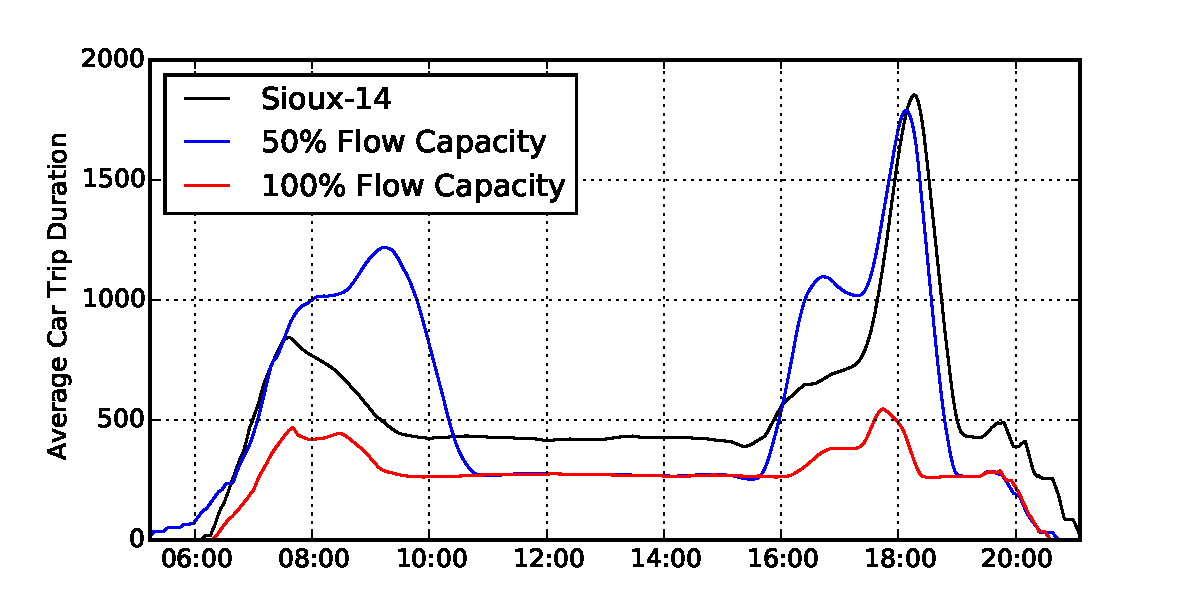
\includegraphics[width=0.9\textwidth]{figures/sioux_times.pdf}
    \caption{Comparison of the average duration of car trips by day time in Sioux-14 and Sioux-16 with 50\% and 100\% flow capacity.}
    \label{fig:sioux_times}
\end{figure}

\begin{figure}
    \centering
    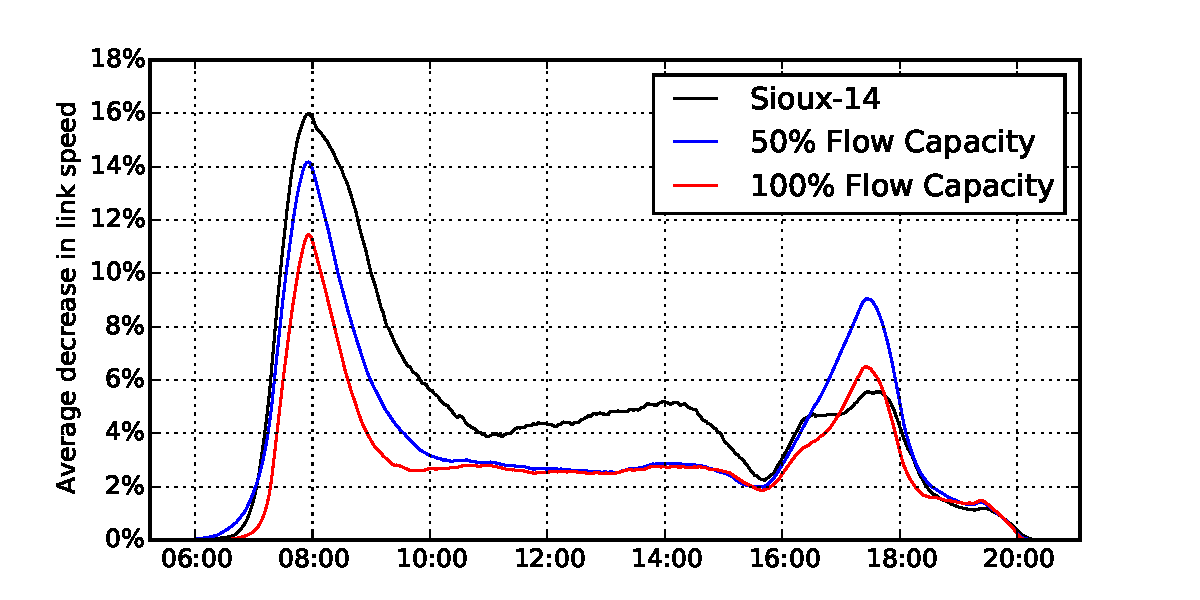
\includegraphics[width=0.9\textwidth]{figures/sioux_speeds.pdf}
    \caption{Comparison of the decrease of link speeds by day time in Sioux-14 and Sioux-16 with 50\% and 100\% flow capacity.}
    \label{fig:sioux_speeds}
\end{figure}


\begin{table}[ht]
\centering
\caption{Comparison of Sioux-14 and Sioux-16 in terms of travel measures. The respective
distances and travel times of the walking legs to and from public transport facilities
are included in the measures for public transport}
\label{tab:sioux}
\begin{tabular}{@{}lrrrr@{}}
\toprule
\textbf{Scenario}                  & \multicolumn{1}{c}{Sioux-14} & \multicolumn{1}{c}{Sioux-16} & \multicolumn{1}{c}{Sioux-16} & \multicolumn{1}{c}{Sioux-16} \\
Flow Capacity                      & \multicolumn{1}{c}{}         & \multicolumn{1}{c}{50\%}     & \multicolumn{1}{c}{70\%}     & \multicolumn{1}{c}{100\%}    \\ \midrule
\textbf{Travel Distances {[}km{]}} & \multicolumn{1}{l}{}         & \multicolumn{1}{l}{}         & \multicolumn{1}{l}{}         & \multicolumn{1}{l}{}         \\
Car                                & 5.30                         & 3.79                         & 3.74                         & 3.70                         \\
Walking                            & 1.31                         & 1.29                         & 1.27                         & 1.26                         \\
Public Transport                   & 3.73                         & 3.82                         & 3.86                         & 3.89                         \\
(Transit Walk)                     & 1.31                         & 0.53                         & 1.28                         & 1.28                         \\\midrule
\textbf{Travel Times {[}mm:ss{]}}  & \multicolumn{1}{l}{}         & \multicolumn{1}{l}{}         & \multicolumn{1}{l}{}         & \multicolumn{1}{l}{}         \\
Car                                & 11:56                        & 08:39                        & 06:59                        & 05:08                        \\
Walking                            & 26:16                        & 25:48                        & 25:19                        & 25:08                        \\
Public Transport                   & 32:37                        & 29:05                        & 28:32                        & 28:14                        \\
(Transit Walk)                     & 24:05                        & 21:50                        & 21:55                        & 21:59                        \\\midrule
\textbf{Mode Shares}               & \multicolumn{1}{l}{}         & \multicolumn{1}{l}{}         & \multicolumn{1}{l}{}         & \multicolumn{1}{l}{}         \\
Car                                & 63.57\%                      & 63.23\%                      & 64.84\%                      & 65.71\%                      \\
Walking                            & 9.29\%                       & 7.50\%                       & 6.80\%                       & 6.56\%                       \\
Public Transport                   & 27.14\%                      & 29.27\%                      & 28.36\%                      & 27.72\%                      \\ \bottomrule
\end{tabular}
\end{table}

%\FloatBarrier
%\hspace{1cm}
 \FloatBarrier \pagebreak
\section{Dynamic Agents in MATSim}
\label{sec:dynagent}

In order to allow for dynamic behaviour in MATSim, several approaches have been
proposed. Mainly the decision on which option is best usually depends on what a
level of complexity in the behaviour is needed.

A simple version of dynamic behaviour is implemented in the public transport
extension, where passenger agents are saved in a list, as soon as they reach the
link in the network, where they should be picked up by a public transport agent.
As soon as the pt agent (e.g. a bus) arrives at that link, persons from the link
are deregistered from the list and ``teleported'' to the destination stop as soon
as the vehicle arrives there. This setup fits very well into the queue based structure
of MATSim.

An even more dynamic approach is used in the DVRP framework, which will be discussed
in the first part of this section. At the time of this thesis and for the specific
use case of autonomous vehicles some drawbacks will be shown and finally a new
abstraction layer for dynamcally acting agents will be presented, which has been
part of the work for this thesis.

\subsection{DVRP}

The DVRP extension \todo{citation} is designed to provide a level of abstraction to the simulation of
dynamic transport services, such as taxis. Its general structure is quite flexible,
so that it is easy to implement for instance electric vehicles \todo{citation} (which need to recharge
at some point during the simulation) or taxis, which are roaming randomly through
the cities and serving concrete requests when they are made by passengers \todo{citation}.

However, this flexibility comes with a cost. The architecture of DVRP basically
circumvents the efficient queue simulation of MATSim for activities. While ``normal''
agents are simulated as described before, dynamic agents (DynAgents) have two
modifications:

\begin{description}
\item[Legs] are sent to the conventional Netsim. However, agents have the ability
to change their paths dynamically, i.e. one can modify the route of the agent
during the simulation steps and the next time the Netsim wants to move the agent
or checks whether the agent should arrive at the current link, its response is
calculated from the updated path.
\item[Activities] are simulated separately from the non-dynamic agents. As soon
as a DynAgent starts an activity it is added to a list of active agents. In each
simulation step a specific callback for each of those agents is called and then
it is checked whether the agent wants to end this activity or not.
This polling approach, as depicted in \cref{fig:polling}, makes sure that it is
not necessary to know when an activity (for instance a taxi waiting for any
requests) should end or how long it should take. On the other hand, this approach
is much more computationally expensive than the efficient queue simulation.
Given that the simulation is done on a second-by-second basis, an activity that
would take one hour, would cost only one insert and one lookup on the acitivty queue.
In the polling approach it costs 3600 calls to the simulation step callback (even
if it does not actually compute anything, thise adds a computational overhead) and
3600 checks whether the activity should be ended.
\end{description}

So far, DVRP has been successfully applied to a number of projects \todo{cite},
though their overall usage of MATSim was different. For instance, in \citet{Bischoff2016}
a study on autonomous vehicles has been done, where the demand in Berlin has been
obtained using an ordinary MATSim simulation. Then the link speed of the underlying
network have been modified, to resemble the traffic situation in a congested
situation and then \textit{only} autonomous vehicles have been simulated. This
means that the simulation could be run once and the results were obtained, because
only the QSim was used and not the evolutionary learning of MATSim.

However, in the project of this thesis, autonomous vehicles should be tested in
an existing multi-modal scenario, where the evolutionary learning is necessary
in order for the agents to arrive at their quasi-optimal mode choices. So if
\citet{Bischoff2016} mentions computational times of 20h for a large number of agents,
it is a measure for one iteration in the evolutionary algorithm. For the scenarios
that will be tested here, a number of 100 iterations still does not reach a satisfactory
equilibirum, though having a theoretical computational time of 2000h, in the case
of the given paper.

Measurements have been made to determine, how much the combination of executing
an empty simulation step for an agent and the execution of an activity callback
that always lets the agent stay in an activity would cost in terms of execution
time on the platform that has been used throughout the thesis. The final results
gave an average time of 25ns. So simulating for instance 8000 agents for a common
time of 30h, would lead to an execution time of:

\begin{equation}
T_{30h} = \underbrace{25}_{\text{Nomial}} \cdot \underbrace{3600 \cdot 30}_{\text{One day in seconds}} \cdot \underbrace{8000}_{\text{Agents}} = 21.6s
\end{equation}

For the whole MATSim simulation, this needs to be multiplied by at least 100 iterations,
so that the overhead of a simulation of 8000 agents doing nothing would already
reach a computational overhead of

\begin{equation}
T_{sim} = 21.6s \cdot 100 = 36min
\end{equation}

Furthermore, while working with DVRP it has been found that the provided examples
for DVRP were not fully compatible with parallelized computation in the Netsim,
which would have lead to a neglect of a good way to improve the computational
performance of the simulation. However, it seems like this problem has been fixed
in the latest version of DVRP by the time of the writing of this thesis.

As a summary, one can say, that DVRP allows for a great freedom in simulating
dynamic behaviour and its structure and signaling flows are very straight-forward
and easy to work with. However, for the purpose of simulating large nubmers of
autonomous vehicles in the whole MATSim with large numbers of iterations, it would
be beneficial to find more efficient ways for the simulation.

\begin{figure}
    \centering
    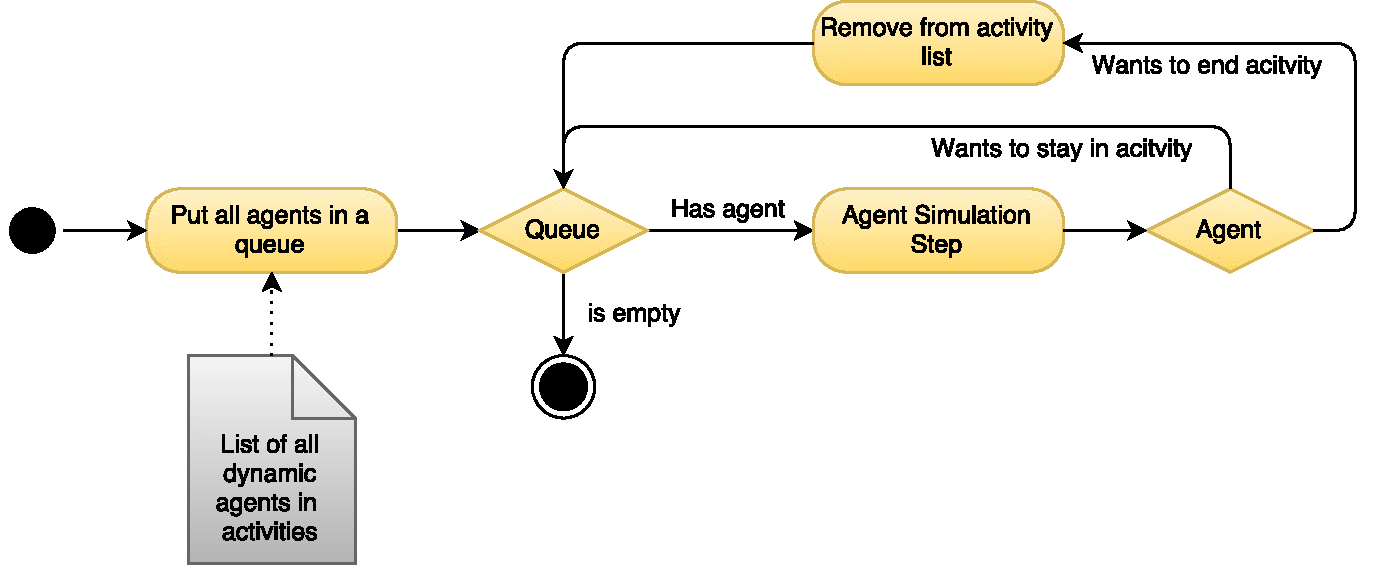
\includegraphics[width=1.0\textwidth]{figures/polling.pdf}
    \caption{Polling approach of the DVRP framework}
    \label{fig:polling}
\end{figure}

\subsection{The AgentLock framework}

As an alternative to the simulation of dynamic agents using DVRP, the AgentLock
framework has been developed as part of this thesis. It tries to combine the advantages
of a queue simulation while providing as much flexibility as possible to create
rich dynamic agent behaviours in MATSim.

The basic idea is as follows: Usually agents in MATSim do not need a lot of processing
power, i.e. the per-agent simulation step of DVRP is hardly ever used and can usually
replaced by some callbacks and event handlers outside of the actual agent simulation.

Furthermore, this means that an activity basically just means that an agent is residing
at a certain position in the network and not taking part of the network. So an
activity for an agent is just keeping the agent back from joining the traffic network
again after a certain time or event.

With this idea in mind, three different types of ways to ``lock'' an agent into
an activity have been proposed:

\begin{description}
    \item[Blocking] activities will just let the agent reside in this activity until
    it is released through a call from outside.
    \item[Time-based] activites are the ones from the basic MATSim simulation: They
    have a certain duration and therefore a fixed end time.
    \item[Event-based] activities let the agent reside in the activity until a certain
    event happens.
\end{description}

The heart of the AgentLock extension is the LockEngine. Whenever it encounters an
agent that wants to start a blocking or event-based activity, it is removed from
the simulation and only added back again as soon as this happens manually or the
event occurs. Then it either is passed to the ordinary Netsim or the next activity
is starts, just as requested by the agent logic.

For time-based activities a similar approach to the activity queue for ordinary
agents is taken. The first idea that would come to one's mind is to order the
agents by the end of their activity and as soon as there is a change in plans,
remove the element from the priority queue and add it back at a certain position.

Compared to DVRP, where a change of plans would cost nothing, here this would lead
to an overhead of $\mathcal{O}(\log n)$ and $\mathcal{O}(n)$ for these operations \citep{JavaPQ}.
So it is neccessary to weigh the overhead of the polling in DVRP against the overhead
of the rescheduling, which mainly depends on how often such reschedulings appear. In
the concrete example of autonomous taxis, this itself depends directly on the travel
demand.

\todo{cite sth here for the PQ? JavaDoc?}

If one sacrifices increasing memory consumption for the sake of having a faster
computational time, this setup can be improved further, as done for the AgentLock
framework. Here, everytime a time-based activity is started, a handle to the
corresponding agent is saved into the priority queue, ordered by the end time of
that activity. Furthermore an indicator is saved, whether the handle is still valid.
So if in the meatime (i.e. before the end of the activity has been processed) the
plan is changed, this handle will be invalidated and it will simply be ignored
when processing the priority queue.

So the whole process works as follows: In every simulation step the top element of
the priority queue is checked. If it is scheduled for the current or a past time
step, it is processed. This means if it is still valid, the agent is ``woken up''
from its current activity and the next state (acitivty or leg) is computed. Afterwards,
or if the handle already had been invalidated, the processing continues with the
updated top element of the priority queue. This process is also shown in figure
\cref{fig:agentlock}. \todo{Create figure, or maybe not necessary?}

The main advantage of this setup is, that elements are only removed at the top
of the queue, which is significantly less expensive than removing elements at
arbitrary positions within the queue.

Furthermore the AgentLock framework provides methods for dynamically ending legs
and it has been made sure that all the functionality has a high degree of compatibility
with the existing parts of MATSim, such as the multi-threaded Netsim.

\subsection{AgentFSM}

While the AgentLock extension mainly provides an abstractionl layer for the dynamic
rescheduling of activities and legs, another layer has been developed, which is
loosely resembling a finite state machine \todo{cite}, tailored towards agents in
MATSim.

In this framework all the activities and legs are predefined states in a finite
state machine and the transitions from one step to another can either be triggered
manually (which is the \textit{blocking} lock from above), by time (\textit{time-base lock})
or by an event (\textit{event-based lock}).

The main task of the AgentFSM framework is to encapsulate common programming steps
when designing dynamic behaviour in MATSim. This means that one usually just has
to define which states the behaviour is built of and how the transition from one
to another works. All of this functionality is provided with a simple programming
interface.

In more detail, each state is either an LegState or ActivityState. For each state
an \textit{enter} callback exists, which the programmer can use to execute arbitrary
code. It needs to return how this state is locked from the three options above or
either issue a direct switch to another state.

As soon as the state is ended due to the above conditions, the \textit{leave} callback
of a state is called, which must return to which next state the simulation should
switch.

The concrete impementation for the autonomous vehicles will be discussed in \cref{sec:avmodel}.

\subsection{Comparison}

An implementation of autonomous vehicles in DVRP has been compared to the implementation
of the AV model developed in \cref{sec:avmodel}. Basically, a specific number $n$ of
autonomous vehicles are created and put into a queue. As soon as an agent wants to
start a leg using an AV, the top element of the queue will drive to that position,
pick up the passenger, bring him to the final destination and drop him off. Then
the AV will be added back to the end of the queue. This dispatching algorithm is
quite inefficient in most of the cases, but sufficient to do investigations in terms
of computational time for the two implementations, since the behaviour is equal and
easily understandable.

First, simulations with $n=2000, 4000, 8000$ have been done on the Sioux Falls scenario, which
will also be described in detail in \cref{sec:avmodel}. What can be seen in \cref{fig:dvrpfsm}
is the share of AV legs of the total number of trips and the associated computation
time. For a large range of shares the implementation using AgentLock and AgentFSM (solid)
is much faster than the coresponding DVRP implementation (dashed). In fact, for $n=8000$
only at a (quite unrealistically big) share of 70\% DVRP starts to be more efficient.

Important to notice is that the performance of DVRP stays roughly the same over
the whole range of shares. This is due to the fact that all 8000 AVs are simulated
in every single time-stpe, no matter if they are active or not. In the AgentLock
implementation, however, agents are only simulated if they are really in use. At
70\% though, when the reschedulings of used AVs are getting to frequent, the repeated
queue operations get more expensive than the polling and DVRP gets more efficient.

As a result, one can say that the FSM implementation is usually more efficient than
the DVRP version. For increasing fleet sizes, this is even more true, since the
roughly constant computation itme for DVRP will increase linearly with $n$, moving
the crossing in \cref{fig:dvrpfsm} further towards 100\%. On the contrary, if only
small fleet sizes are used, the range of leg shares with FSM in favor will get
smaller and smaller, because reschedulings get to frequent compared to the number
of AVs.

\begin{figure}
    \centering
    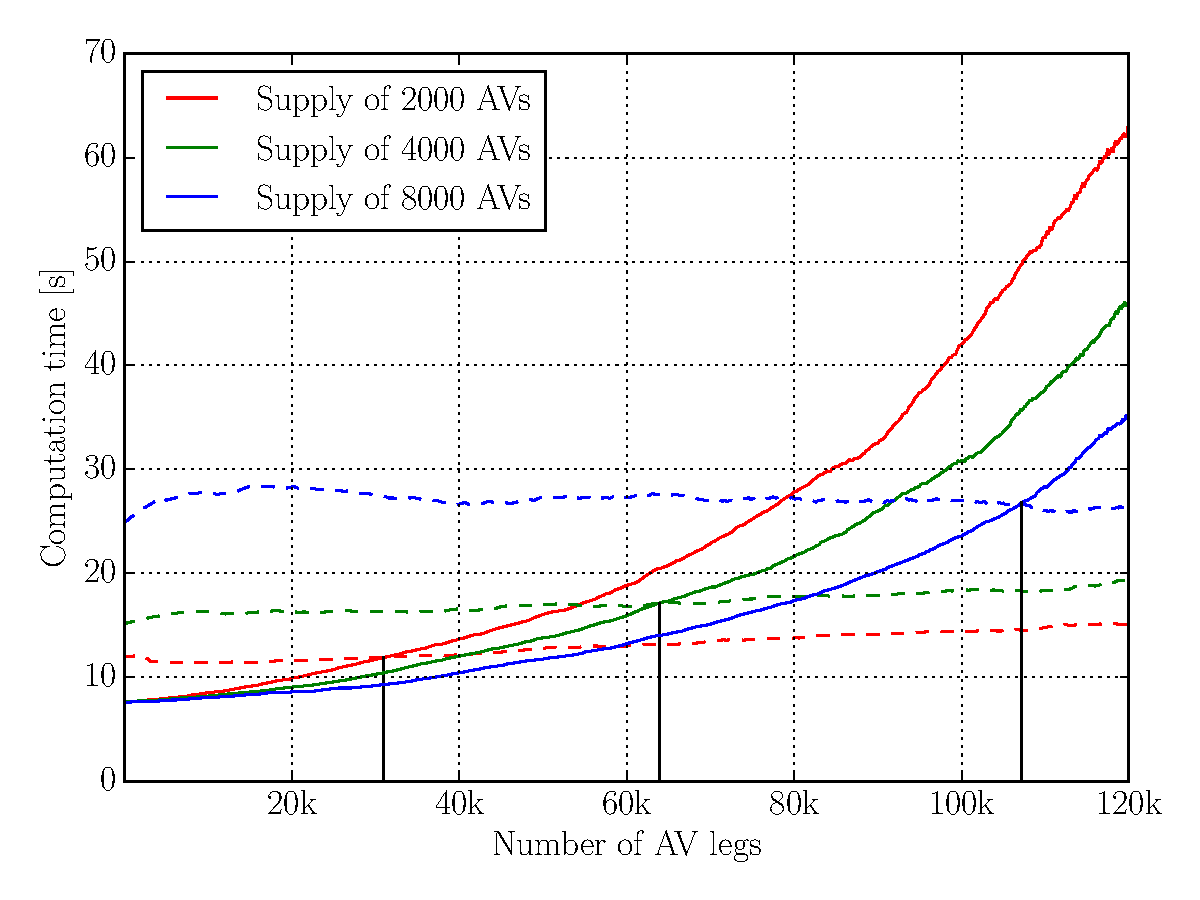
\includegraphics[width=0.7\textwidth]{figures/dvrp_fsm.pdf}
    \caption{Comparison of Mobsim computational time between DVRP and AgentLock/AgentFSM implementation, dependent on share of AV legs. Scenario is Sioux Falls with
    a total number of legs of around 280.000. \todo{Measure again, at least for FSM-8000 for a better plot}}
    \label{fig:dvrpfsm}
\end{figure}

In terms of a multithreaded Mobsim, only tests with the new AgentLock implementation
could be done, as shown in figure \cref{fig:threads}. Obviously, though the improvement
is small, the simulation with two threasd performed best. This shows that it is
actually an advantage to be able to use the multithreaded Mobsim. Similar results
have been found for other scenarios, for instance the optimal number of threads
for the Singapore scenario has been found to be four \citep{Erath2014}.

\todo{For the graphics, explain better what is shown: Time for whole Mobsim; also
explain how the shares are computed?}

\begin{figure}
    \centering
    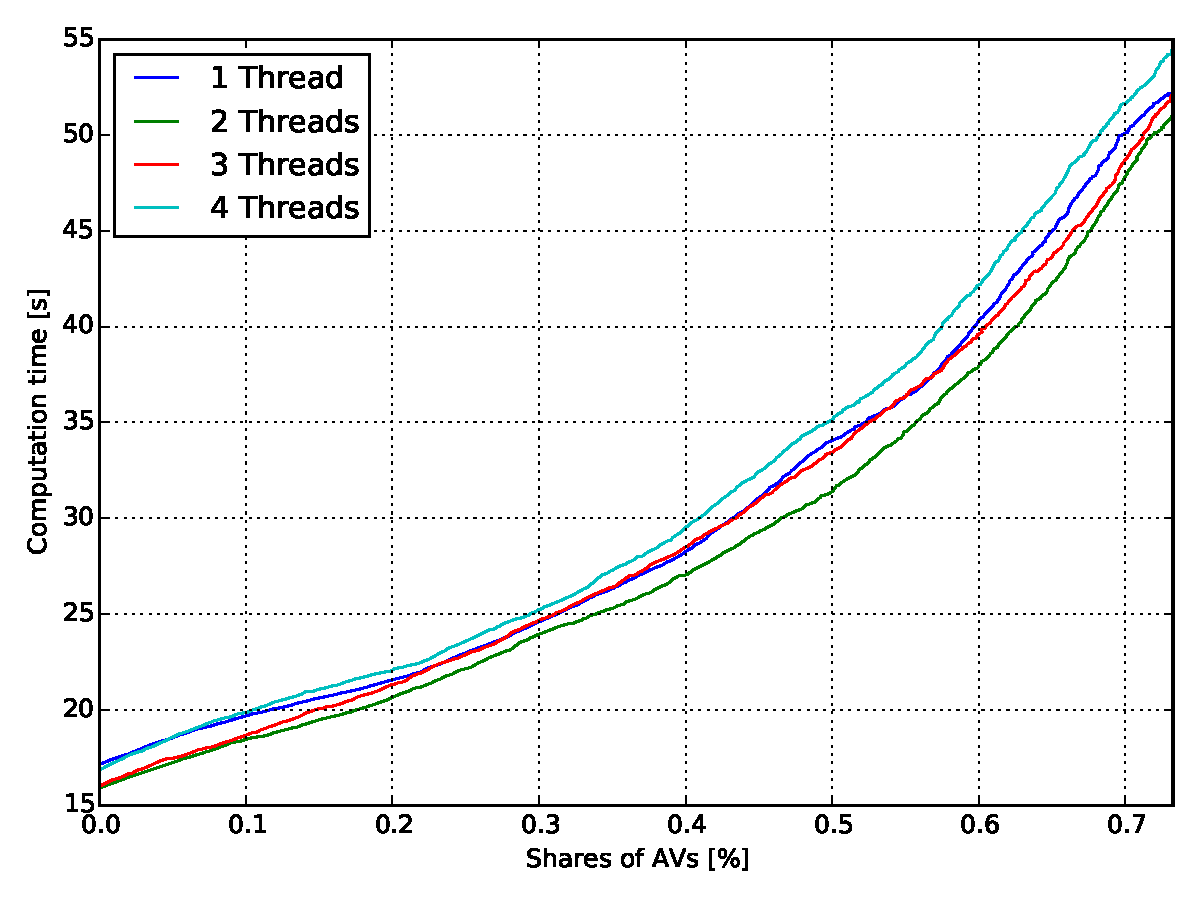
\includegraphics[width=0.7\textwidth]{figures/threads.pdf}
    \caption{Comparison of different numbers of threads for the Mobsim with the AgentLock implementation}
    \label{fig:threads}
\end{figure}


\todo{add comments on how to design a dynamic agent framework in an adaptive way, using each strategy when it makes more sense}
\todo{should be very easy to implement. maybe even present some measurements as an outlook, if there is enough time to implement
a simple version (at least a hard switch to polling instead of queueing)}
 \FloatBarrier \pagebreak
\section{Autonomous Taxi Fleet Model}
\label{sec:avmodel}

Simulating autonomous taxi services in MATSim requires the implementation, but
even more so a concise planning and definition of how the exact behaviour of
those agents should look like. This will be the first part of this section. Then,
when it is known how those agents can be simulated the next question is how they
should be dispatched for the requests of passengers and finally it has to be decided,
where the autonomous taxis are placed on the network at the beginning of the simulation.
These question will be answered in the second and third part of this section.

\subsection{Agent Behaviour}

The behaviour of an autonomous taxi is not a lot different from an ordinary one,
except that there is no need to roam through the city to find new customers. Therefore,
the AV behaviour presented here is mainly inspired by the model in \todo{cite}, where
ordinary taxi services have been simulated.

The behaviour of an autonomous taxi agent can be described in terms of a task life
cycle. When the agent is not in a task, he is in idle mode, basically (for the basic
model) meaning that he will just stay at the current position and wait for further
instructions. The following steps in the life cycle are depicted in \cref{fig:avstates}.

\begin{enumerate}
\item \textbf{Pickup Drive} is the phase where the AV has got a task and is moving
to the requested pick up location. If the AV is already at the right location, this
point can be skipped, otherwise it represents a leg driving from the current position
to the pickup location.
\item \textbf{Waiting} is the phase in which the AV has arrived at the pickup
location, but the passenger is not there yet. This can only happen if passengers
request cars in advance, prior to the time when they actually want to be picked
up. If the passenger is already present at the time of the arrival at the pickup
location, this state can be skipped.
\item \textbf{Pickup} is the state in which the passenger is picked up. It is
modelled as a fixed time, e.g. one minute and started as soon as both the AV
and the passengers are present at the pickup location.
\item \textbf{Dropoff Drive} represents the leg going from the pickup location to
the dropoff point.
\item \textbf{Dropoff} is the point where the passenger leaves the vehicle. Again,
this is modelled as a fixed time interaction.
\item \textbf{Idle} is the final (and initial) state of the AV life cycle. At this
point the AV will just wait until it receives a new task to pick up another passenger.
\end{enumerate}

The states described above fit very well to the distinction of Activities and Legs
in MATSim as well as to the structure of the AgentFSM framework, which has been
developed for this purpose. Resulting from this behavioural model, a couple of
parameters end implementational questions arise, that can be configured accordingly:

\begin{description}
\item[The Idle behaviour] for the basic model just means that the AV will stay at
its last position. Future extensions could make use of parking facilities or do
an intelligent repositioning to improve the overall performance of the service.

\item[Pickup and Dropoff duration] need to be specified. In accordance with
\todo{cite}, $t_{pickup} = 120s$ and $t_{dropoff} = 60s$ have been chosen. The time
used for the pickup action will not be counted as waiting time (which, in turn,
would be penalized through the marginal utility of waiting as described before).

\item[The routing] of the legs of the AVs is done semi-dynamic, as soon as a
request is issued. What this means is that only the traffic situation of the
previous iteration is taken into account. During an iteration the average travel
speeds for all network links are tracked in a number of time bins throughout the
day and used in the next iteration. In order to smoothen the measurements and
allow for a faster convergence of the scenario, the measured travel times are
averaged with those of the previous iteration.
For the routing through the network a plain
Dijkstra algorithm is used, with the shortest path being the one with the shortest
expected driving time with respect to the inferred travel speeds. This
also means that the current traffic situation, which might slow down some links,
is not taken into account directly, but only indirectly from previous knowledge.
Parameters that are involved in the routing are the number of time bins per day
and the interpolation factor when averageing over the previous iteration.
\todo{Explain that this has been implemented due to overcongestion when too many
AVs are used, which would take the exact same main routes. The averaging over
previous iterations can also be explained further in terms of dynamical system
/ random process properties, i.e. it is a stable AR(1) process.}
\end{description}

\begin{figure}
    \centering
    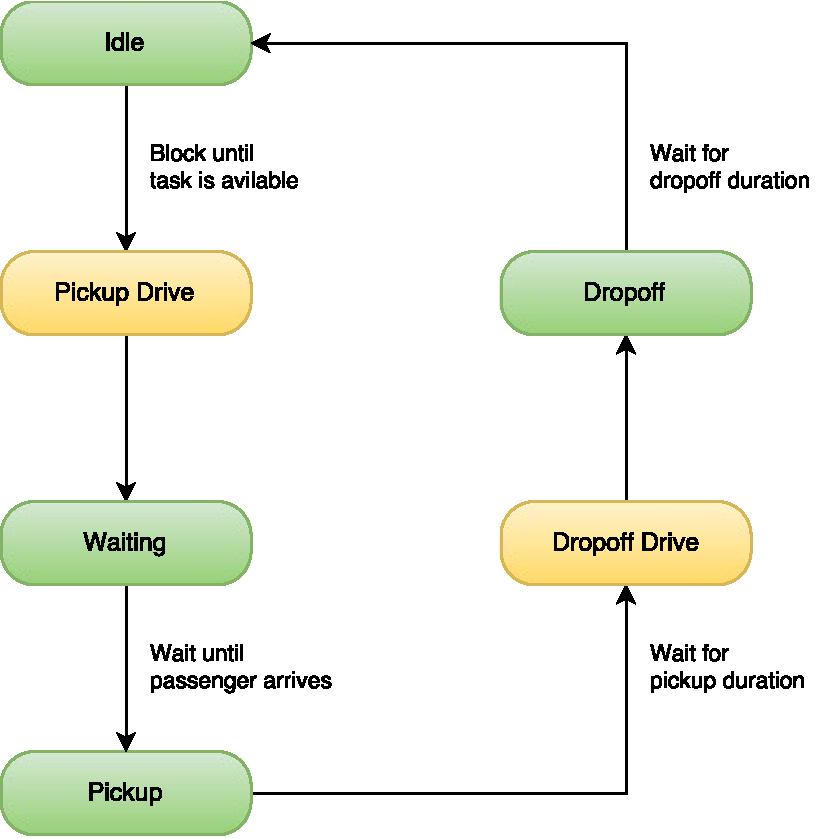
\includegraphics[width=0.7\textwidth]{figures/avstates.pdf}
    \caption{State chart of an AV agent. Activity states are displyed in green, while Leg states are yellow.}
    \label{fig:avstates}
\end{figure}

\subsection{Dispatcher Algorithm}

The dynamic dispatching of taxi vehicles is quite a complex scheduling problem,
which is quite hard to solve or needs numerous asumptions to be feasible. In
general, the problem will be a NP hard and heuristical solution strategies need
to be applied if fast solutions are needed. An overview, as well as a proposed
heuristic algorithm can be found in \citet{Maciejewski2015, Bischoff2016}.

The algorithm can be described in two different states:

\begin{description}
\item[Oversupply] occurs when there are more available autonomous vehicles than
requests. This means that each request can be assigned without delay. In that case,
as soon as a request arrives at the dispatcher, the closest vehicle to this request
is searched and assigned to serve the customer.
\item[Undersupply] is the case when all autonomous vehicles are occupied. In that
case requests will stack up, which cannot be handled immediately. In this case the
algorithm works the other way round: As soon as an autonomous vehicle gets available,
it is dispatched to the closest request.
\end{description}

According to the beforementioned papers this strategy gives a near-optimal solution,
although providing fast computational times.

The implementation for this thesis is based on a spatial relaxation of the traffic
network. This means that a grid with a specific resolution in x and y is fitted
over the links. One of these grids saves the locations of all the available AVs,
while another grid saves the locations of all open requests. Because the grids have
a fixed structure, finding the closest AV or request is quite simple, since each
position in x and y belongs to one specific cell of the grid. If no option is found
in a certain cell, the search continues with all cells in its Moore neighborhood
(all 8 surrounding cells). If this still gives no result, the radius is increased
and so forth. When specifiying ``find at least $K$ hits'' as a stop criterion for
a search this resembles an approximate K-nearest-neighbor search based on a $L_1$
norm due to the grid character.
The procedure is depictred in \cref{fig:gridsearch}.

\begin{figure}
    \centering
    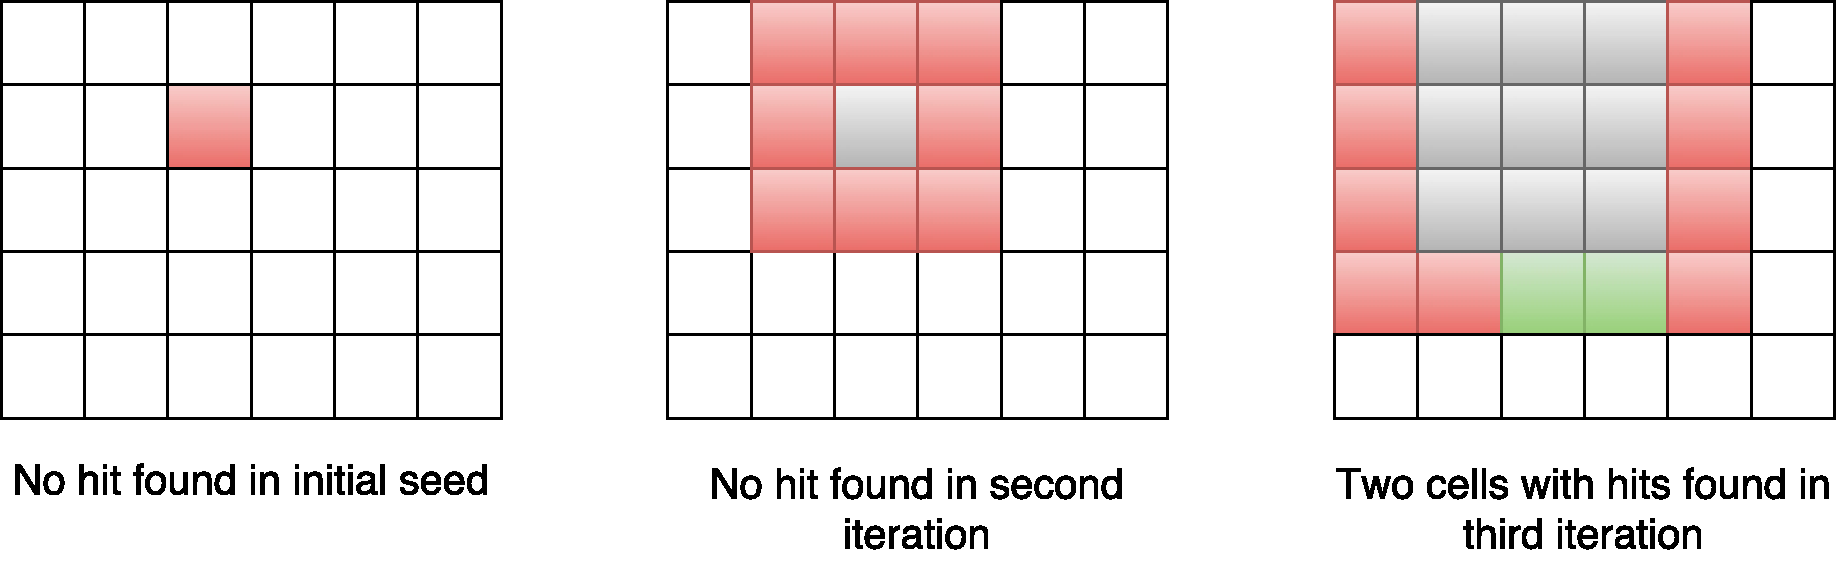
\includegraphics[width=1.0\textwidth]{figures/gridsearch.pdf}
    \caption{Schematic grid search algorithm for the dispatcher}
    \label{fig:gridsearch}
\end{figure}

This search algorithm imposes new parameters to the implementation, which basically
are the cell counts in horizontal and vertical direction. Depending on the topology
of the network, different parameters might be more efficient. If the grid is chosen
to be too dense, many iterations are needed in the algorithm, while a too sparse one
in the extreme case can lead to finding most of the items in only single cell.

In fact, for some topologies it might probably be more efficient to use different
data structures like a binary tree or quadtree to improve the search procedure.
Also more elaborate network search algorithms could be used, which make direct use
of the topology. \todo{cite example maybe}

\todo{Explain how this has been parallelized! Show spoeed improvement!}

For the Sioux Falls scenario it has been tested which impact the choice of the grid
size has on the results. I \cref{fig:gridsize} one can see that very high resolution
grids ($n=200$) lead to a great increase in computational time, due to the necessary
``expansion'' of unoccupied cells, as described above. On the contrary, very low
grid sizes lead to very poor results in terms of the overal average travel time of
the agents, because just selecting a random agent from one of a few cells is basically
just random assignment. A good value for the Sioux Falls network has been found to
be $n=20$, which is computed fastest over the whole range of shares and furthermore
does a good job in decreasing the overall travel time.

\begin{figure}
    \centering
    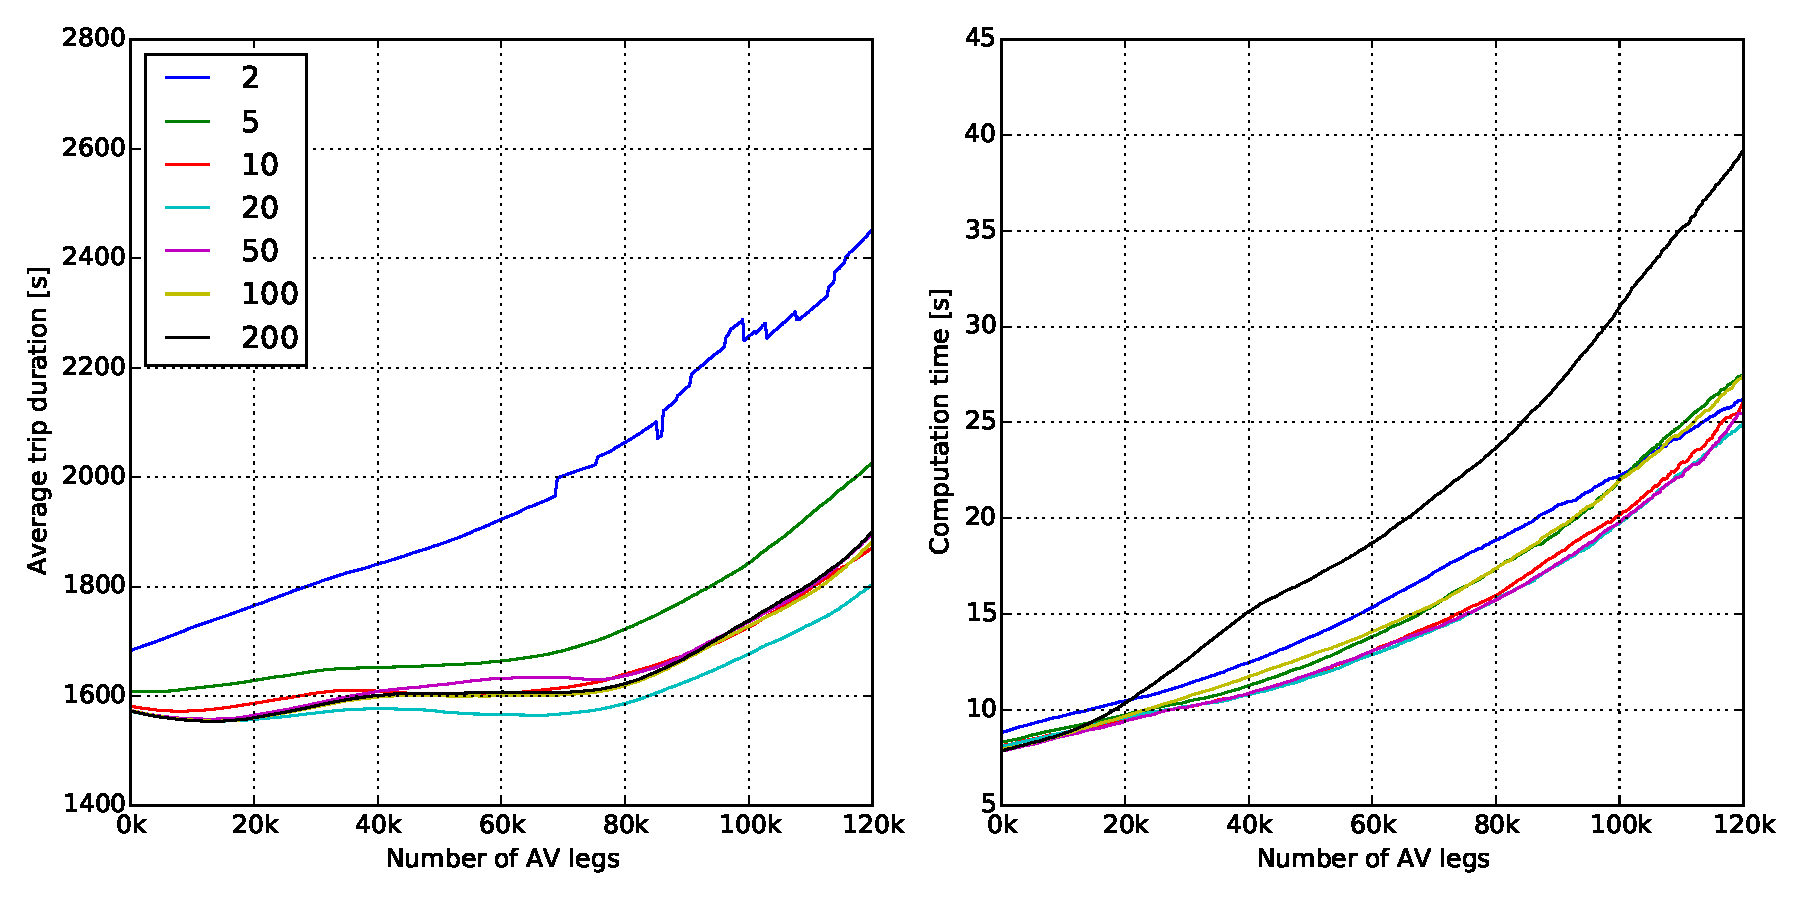
\includegraphics[width=1.0\textwidth]{figures/gridsize.pdf}
    \caption{Performance of different grid sizes in the dispatching algorithm for Sioux Falls}
    \label{fig:gridsize}
\end{figure}

Further improving the dispatching process, the routing has been parallelized. When
the dispatcher is called one per iteration, all the assignments between autonomous
taxi agents and passengers are cached to be processed while the network simulation
of the next iteration is running. Only then, so after one iteration, the dispatcher
waits for all running routing jobs to finish and notifies the agents. This way all
the expensive routing through the network can be done in parallel to the Netsim.
\Cref{fig:routers} shows the impact of adding this feature: While only applying
one parallel router there is already a huge increase in computational performance
compared to the serial processing of the routing tasks. As soon as more routers
work concurrently, this performance is even improved. However, as usual there is
the point where managing the parallelization adds more overhead to the simulation.
For the given scenario a number of routers of $2$ seems to be a reasonable choice.

The parallelization of the dispatcher could be pushed even further. Next to the
routing the actual assignment is the other expensive component in the algorithm.
However, it would probably be hard to parallelize, because concurrent workers
would need to access the same grid structures. The overhead of managing which
worker has access is likely to very fast add more overhead than improvement to
the simulation. One could, however, put the whole assignment process as a serial
procedure in parallel to the Netsim, as done with the routers. This could be a
promising approach of pushing the performance of the simulation even further.

\begin{figure}
    \centering
    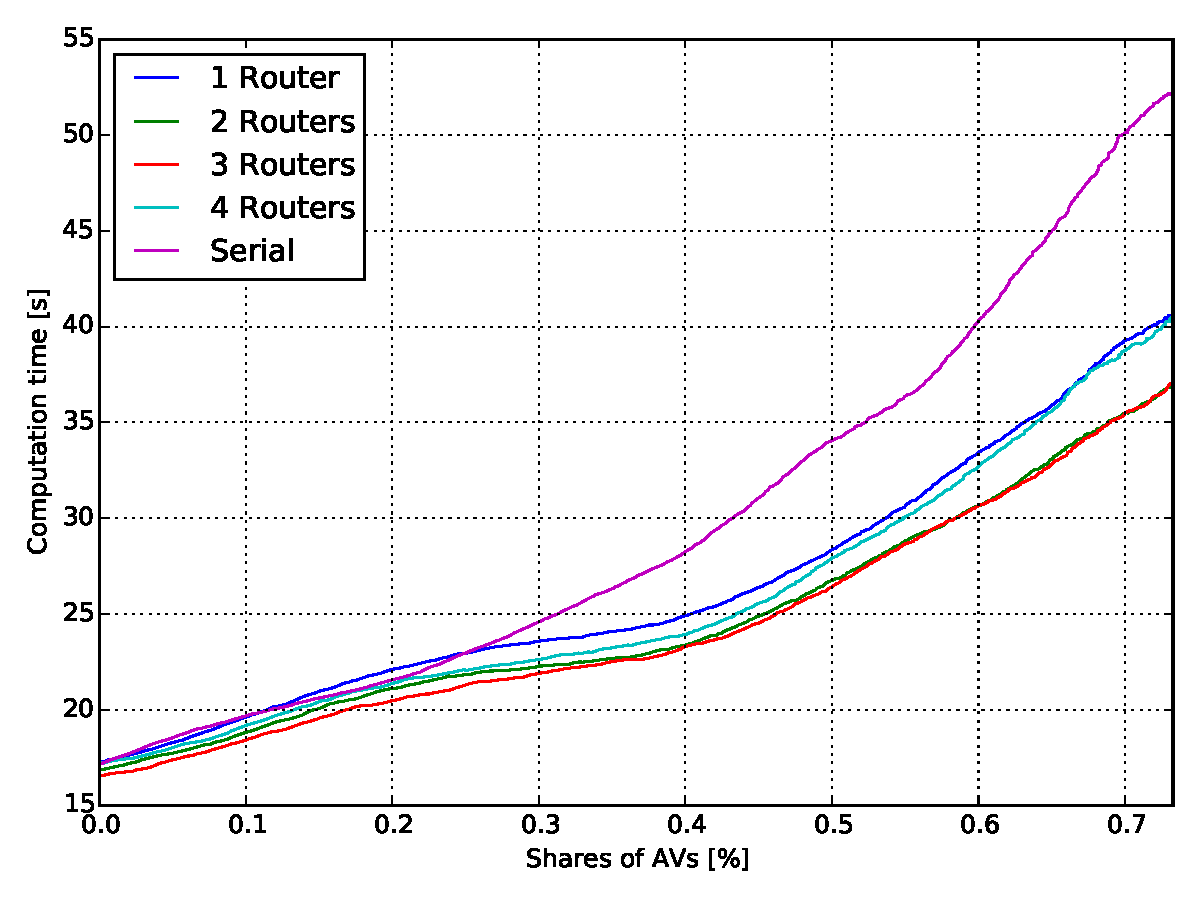
\includegraphics[width=0.7\textwidth]{figures/routers.pdf}
    \caption{\todo{todo}}
    \label{fig:routers}
\end{figure}

\subsection{Distribution Algorithm}

At the beginning of a day simulation MATSim all the $n$ available AVs must be placed
somewhere in the network. Two simple distribution algorithms have been implemented
for the purpose of testing in this thesis.

The first one is \textbf{Random Distribution}. Here $n$ links are chosen randomly
from all available network links. While this is an easy distribution strategy for testing,
it create a quite unrealistic scenario. Obviously, in a real AV service, vehicles
would be relcoated over night, such that they can serve as many passengers as
possible during the morning peek.

Therefore a more elaborate distribution strategy has been implemented, which should
lead to more realistic results. Basically one can define a density over the network,
such that every link has a certain probability to get an AV assigned. Then, in $n$
steps, the $n$ available AVs are added to a link dependent on the assignment
probability.

This probability density can be based on many factors. The ones that are implemented
for this thesis are:

\begin{description}
\item[Population density] What is measured here is the population density in terms of
how many people are havingtheir ``home'' activity on a certain link.
\item[AV commuter density] Here for each link it is counted how many people will
have chosen the AV mode for their first leg, i.e. the one that is starting from home.
\end{description}

While the prior one is static, the latter on is dynamic in the sense that for every
iteration in the evolutionary learning, the density will change. So while the
population-density based distribution is a fixed constraint, the latter one captures
the factor of availability. For instance, if there are many agents using AVs in a
certain area, the availability is very high, and thus more people might be inclined
to use it. On the other hand, if availability is low in an area, it might lead to
longer waiting times and people are less likely to use AVs.

While it might be interesting to observe different patterns of availability,
for the first testing purposes the population density is better suited, since a
detailed investigation would need to be done if any results from the AV leg density
come from the mode choice of the agents or of feedback behaviour within the algorithm
itself.

\subsection{Sensitivity Analysis}

\todo{Ongoing. The follwing are just notes.}

Idea is to find the general properties how the demand depends on the
parameters. The idea is that there should be two limiting factors: The utility (depending
on the cost of the AV, the equilibirum will find a certain value) and the supply (
if utility is such good that the AVs go into saturation, the supply level should
dominate the equilibirum).

Some questions:

+ What are the utility values at which the system goes into saturation?
+ How does the supply effect the share of AVs?

For the utility the effects should be quite clear. In some way, giving better
utility to AVs should increase the AV share until it goes into saturation.

For the supply the situation is a bit different. If there are no enough AVs it
will be quite unattractive to use AVs, because one has to wait really long. So
it is likely that there is a threshold, which defines the minimum supply in the
system.

Then again there should be an interplay between utility and supply, because
if one has saturation at a certain utility and then increases the supply, again
going into saturation there are less and less people who are \textit{not} using
AVs, so the increase should have a parabolic shape, while increasing the utility
when the system is not in saturation should show a logistic growth.

In essence, what I'm trying to find out if there is a parametric bifurcation, that
let's changes the eqilibirum dynamcis substantially...

The prupose of all the sensitivity analysis is to get a bit more insight for the
following operator model, because there the variables will be the cost per km
for the operator and the price for the customer, as well as a price per car which
depends on the supply. 
 \FloatBarrier \pagebreak
\addtocontents{toc}{\protect\newpage}
\section{Simulation Results}
\label{sec:results}

Once the simulation model had been established, simulation runs with carefully
defined parameters have been performed. The following sections will give an
overview about the simulation results.

First, a baseline scenario will be defined with the corresponding utility parameters.
The resulting trip statistics and mode choices will be analyzed (\cref{sec:baselinesc}).
In \cref{sec:waitingtimes} different levels of supply will be examined and their
effects on the overall net mileage and waiting times will be shown. \Cref{sec:costs}
shows relevant traffic statistics, such as the AV mode share, in dependency on
the pricing scheme, while \cref{sec:economics} will introduce an operator model
and analyze the profitability of the AV mode from a service provider perspective.

The simulations performed in this chapter have been computed over 500 iterations,
with the innovation of agents' plans being turned off after 420 steps. Generally,
this is a generous setup, since relaxation is usually reached after around 200
iterations. In terms of computation time, the increase was found to be linearly
dependent on the number of AV legs, with an increase of $80\%$ per 100,000 legs
compared to the baseline Sioux-16 scenario without AVs.

\subsection{Baseline Scenario}
\label{sec:baselinesc}

The model with the implementation that has been described in the previous chapters
has been tested on the Sioux-16 network
with a flow capacity scaling of $70\%$ to allow for a reasonable amount of congestion.

The travel disutility parameter has been chosen to be zero, as is the travel
disutility for taking a car in Sioux-16. The reason behind this is that there are
numerous studies indicating positive and negative effects of autonomous vehicles, so
it is hard to decide whether the perception of AVs will tend towards one side or the
other compared to cars.

The constant disutility for cars in the Sioux-14 scenario
has been computed by combining the travel disutility for 10min walking (as to
account for getting to and from a parking lot) and the monetary disutility for
paying \$6 for parking. For the AVs in this simulation it has been assumed that
there is no such additional cost, but a monetary fee per AV trip. This
assumes that a fictitious operator already included the costs of parking into the
pricing scheme (which is reasonable taking the values from actual taxi services).

Since the values in Sioux-14 are based on measurements in Sydney, the current
maximum charges for taxi trips there have been used as a reference \citep{NSW2016}. According to this
source, an initial charge of \$3.60 has been set as the constant disutility per trip, while
the monetary distance factor for AVs has been set to \$2.19 per km. This pricing
scheme has been chosen to allow for a comparison with a service that exists in
reality. As will be shown later on, this setup leads to a surprisingly high share
of the AV mode.

Finally, the disutility for waiting for an AV has been assumed to be the same as
the waiting disutility for public transport from Sioux-14, which itself is just a
vague assumption \citep{Chakirov2014}, but at least allows for a systematic comparison.

\begin{table}[]
\centering
\caption{Baseline Scenario Parameters}
\label{tab:baselineparams}
\begin{tabular}{@{}lll@{}}
\toprule
Parameter                       & Computation & Baseline Value \\ \midrule
Constant Utility per Trip       & $C_{av} = -\beta_m \cdot \$3.60$    & $-0.2232$ \\
Marginal Utility of Travel Time & $\beta_{trav,av} = \beta_{trav,car}$            & $0.0$ \\
Monetary Distance Rate          & $\gamma_{av} = 2.19 \$/km$            &  $0.00219$              \\
\midrule
Marginal Utility of Wait Time   & $\beta_{wait,av} = \beta_{wait,pt}$            &  $-0.18$              \\ \bottomrule
\end{tabular}
\end{table}

Using these parameters, which are summarized in \cref{tab:baselineparams}, the
scenario has been simulated until relaxation. The following paragraphs will show
the respective results in terms of the traffic situation. A sufficiently high
number of available AVs ($N=8000$) has been chosen to show how agents make a choice for taking
an AV based on their utility evaluation.

\subsubsection{Trip Statistics}

\Cref{tab:withwithoutav} shows the basic trip statistics of the case where
AVs have been introduced to the baseline scenario. It can be seen that with the
given utility parameters, the AVs reach a share of around $25\%$ averaged over
the day, mainly decreasing the share of public transport and walking while also
attracting some of the former private car users. Given the quite expensive
price structure for the AV mode, this result is surprising and likely a result
of the calibration of the existing parameters from the Sioux-14 scenario, which
might only be consistent in themselves. Nevertheless, comparisons to this AV baseline
scenario allow for qualitative conclusions regarding the simulation outputs.

Interesting to see is that for public transport and walking agents the travel
distances decreases because relatively long trips in those modes will be replaced
by AVs, thus drawing the average down to shorter trips, while it increases for cars.
Here, mainly the shorter car trips are replaced by AVs.

These results can also be in \cref{fig:modehist_av}, where the distribution of
travel distances by mode is presented. Clearly, AVs act as a competitor towards
public transport there, serving mainly the same range of trips with the assumed
utility parameters.

\begin{figure}
    \centering
    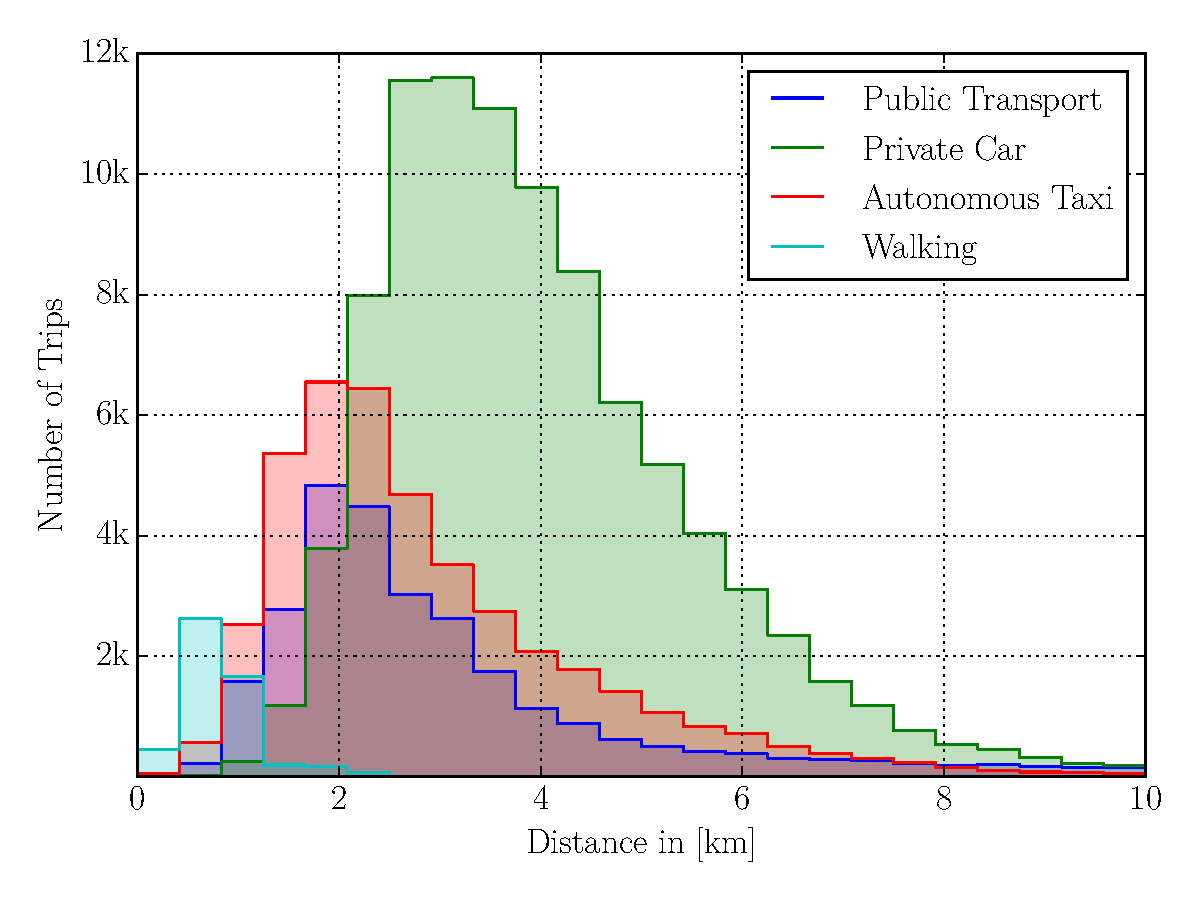
\includegraphics[width=0.9\textwidth]{figures/modehist_av.pdf}
    \caption{Number of trips for each node by traveled distance}
    \label{fig:modehist_av}
\end{figure}

In terms of travel times, it can be seen that there is a slight increase for the car
mode, which stems from the same argument as before. The decrease in travel time for
public transport and walking agents is quite significant, though. For the walking
agents, the change is obvious as described before. The decrease for public transport
can be explained by the switch of agents, who needed to have long walking distances
to the closest bus stop, which is included in the calculation. By only keeping those
agents at using public transport, who live nearby a bus stop, the overall travel
time decreases quite substantially.

% Please add the following required packages to your document preamble:
% \usepackage{booktabs}
\begin{table}[]
\centering
\caption{Traffic measures for the relaxed AV baseline scenario}
\label{tab:withwithoutav}
\begin{tabular}{@{}lll@{}}
\toprule
                                   & \textbf{Baseline} & \textbf{With AV} \\ \midrule
\textbf{Travel Distances {[}km{]}} &                   &                  \\
Car                                & 3.73              & 4.04             \\
Walking                            & 1.25              & 0.82             \\
Public Transport                   & 3.88              & 3.25             \\
Autonomous Taxi                    &                   & 2.94             \\
\textbf{Travel Times {[}mm:ss{]}}  &                   &                  \\
Car                                & 07:20             & 08:07            \\
Walking                            & 25:01             & 16:29            \\
Public Transport                   & 28:48             & 20:41            \\
Autonomous Taxi                    &                   & 10:41            \\
\textbf{Mode Shares}               &                   &                  \\
Car                                & 65.04\%           & 55.08\%          \\
Walking                            & 6.79\%            & 3.08\%           \\
Public Transport                   & 28.17\%           & 16.65\%          \\
Autonomous Taxi                    &                   & 25.19\%          \\ \bottomrule
\end{tabular}
\end{table}

The waiting times for AVs in the baseline scenario are on average around 04:40 min in the morning peak
and 02:55 min in the afternoon, while the daily average lies at 01:40 min. A more
detailed analysis of waiting times is given in \cref{sec:waitingtimes}.

In terms of travel distances the total amount of kilometers driven increased from around 424,000 km in
the baseline to 553,000 km in the AV scenario. The amount of kilometers driven by AVs
is 162,500 km from which around 37,800 are for the purpose of picking up passengers, i.e.
they are unoccupied while covering this distance, which is roughly $23\%$. This is around half
compared to ordinary taxis with 52\% as stated in recent statistics for Oslo \citep{Norway2015}
or around 50\% in Barcelona \citep{Amat2014}.

\subsubsection{Mode Choice}

\Cref{tab:basemodeshares} shows how the mode choice that takes place after AVs
have are introduced. The rows show the original modes while the percentages
indicate how many of the initial users switch to the mode in the column after the
introduction of AVs. What can be seen is that $44\%$ of all initial public transport
users and $56\%$ of all walking people opted for taking an AV while only $14\%$
of car users switch modes. This again shows that with the baseline parameters, AVs rather
work as a competitor against public transport while additionally drawing new adopters
from the walking people. Therefore, this scenario represents the rather unwanted case
where AVs lead to a less optimal situation on the road, leading to more
congestion and less use of collective transportation.

% Please add the following required packages to your document preamble:
% \usepackage{booktabs}
\begin{table}[]
\centering
\caption{Migration matrix showing which agents switched from one mode to another:
The rows resemble the initial choices of the agents while the columns resemble the
mode choice after the introduction of AVs. The percentages denoted how many users
of the original mode switched to another option.}
\label{tab:basemodeshares}
\begin{tabular}{@{}lrrrr@{}}
\toprule
                 & AV & Car     & PT & Walking \\ \midrule
Car              & 13.69\%    & 84.41\% & 1.68\%           & 0.23\%  \\
Public Transport & 44.29\%    & 0.60\%  & 54.91\%          & 0.21\%  \\
Walking          & 56.21\%    & 0.18\%  & 1.38\%           & 42.24\% \\ \bottomrule
\end{tabular}
\end{table}

A further impression on the choice behavior of the agents can be obtained through
\cref{fig:changes_modes}. In the upper plot one can see the public transport trips
in the baseline without AVs (blue), which have not changes during the introduction
of the new mode while the red dots show those combinations of trip duration and
distance in the original scenario, which have changed to AV. Comparing the blue
and red areas it becomes evident that users with rather long trips in terms of
travel time switch to AVs. The green dots show the combinations after the change
has been taken place, i.e. the travel duration and distance in the converted AV
trips. It can be seen that after the introduction of AVs the travel durations
get much less, so for the public transport users, the AV mode is mainly attractive
because it provides shorter net travel durations.

The lower plot in \cref{fig:changes_modes} shows the same arrangement for private
car users. One can see that the switching users (red) are clustered for short trips in
distance and duration. Their travel times, contrary to the public transport users,
increase when using the AVs, indicating that the monetary benefit of using the AV
instead of going on a private car trip (and paying for parking) is stronger than
the desire to have a minimal travel time.

From the utility parameters, one can equate the resulting utility of
a private car and an AV trip with the same distance:

\begin{equation}
C_{car} + \beta_m \cdot \gamma_{car} \cdot d = C_{av} + \beta_m \cdot \gamma_{av} \cdot d
\end{equation}

Solving for the variable distance, one reaches at a critical distance, at which
AV trips should get unfavorable, which is:

\begin{equation}
d_{crit} = 3.05 km
\end{equation}

This value can be observed in \cref{fig:changes_modes}, where in the lower plot
a strict barrier can be seen at this distance.

\begin{figure}
    \centering
    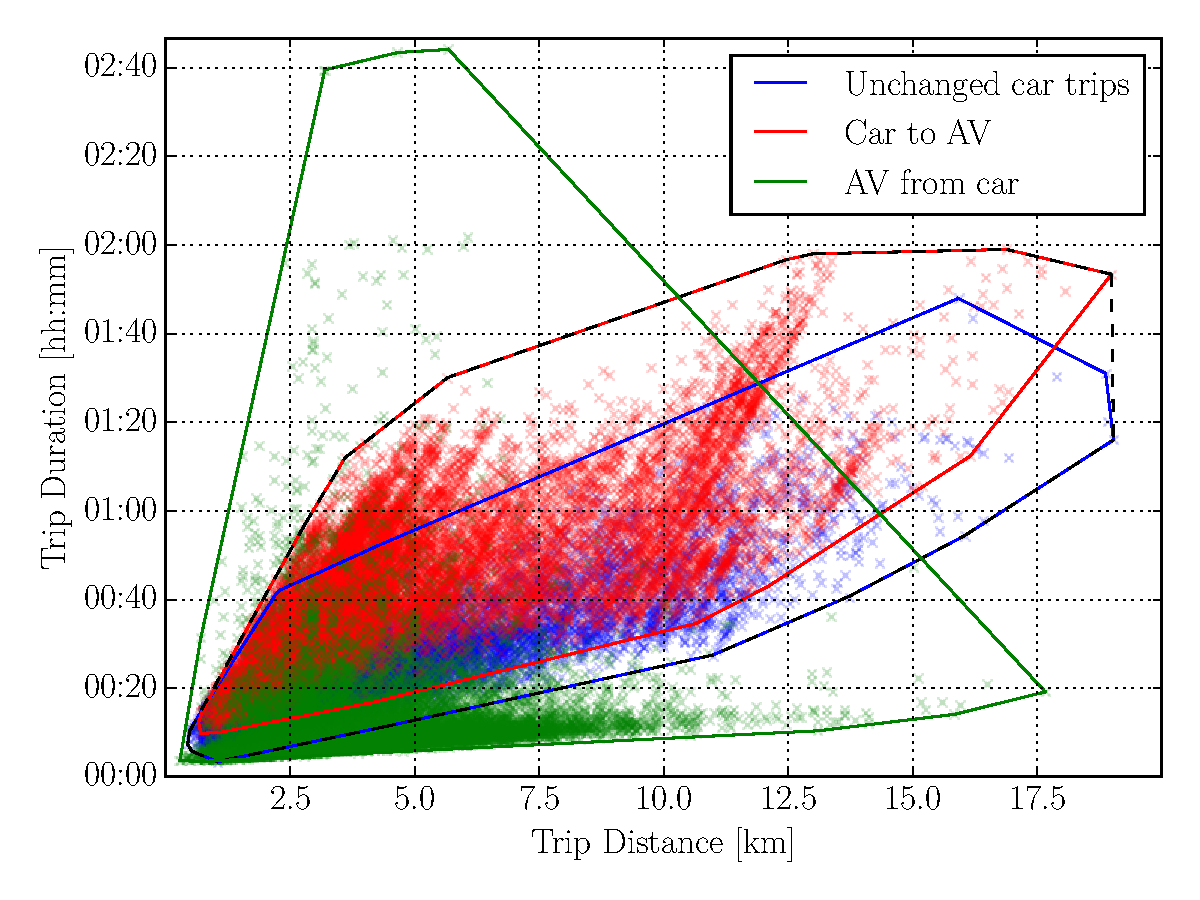
\includegraphics[width=0.9\textwidth]{figures/changes_pt.pdf}
    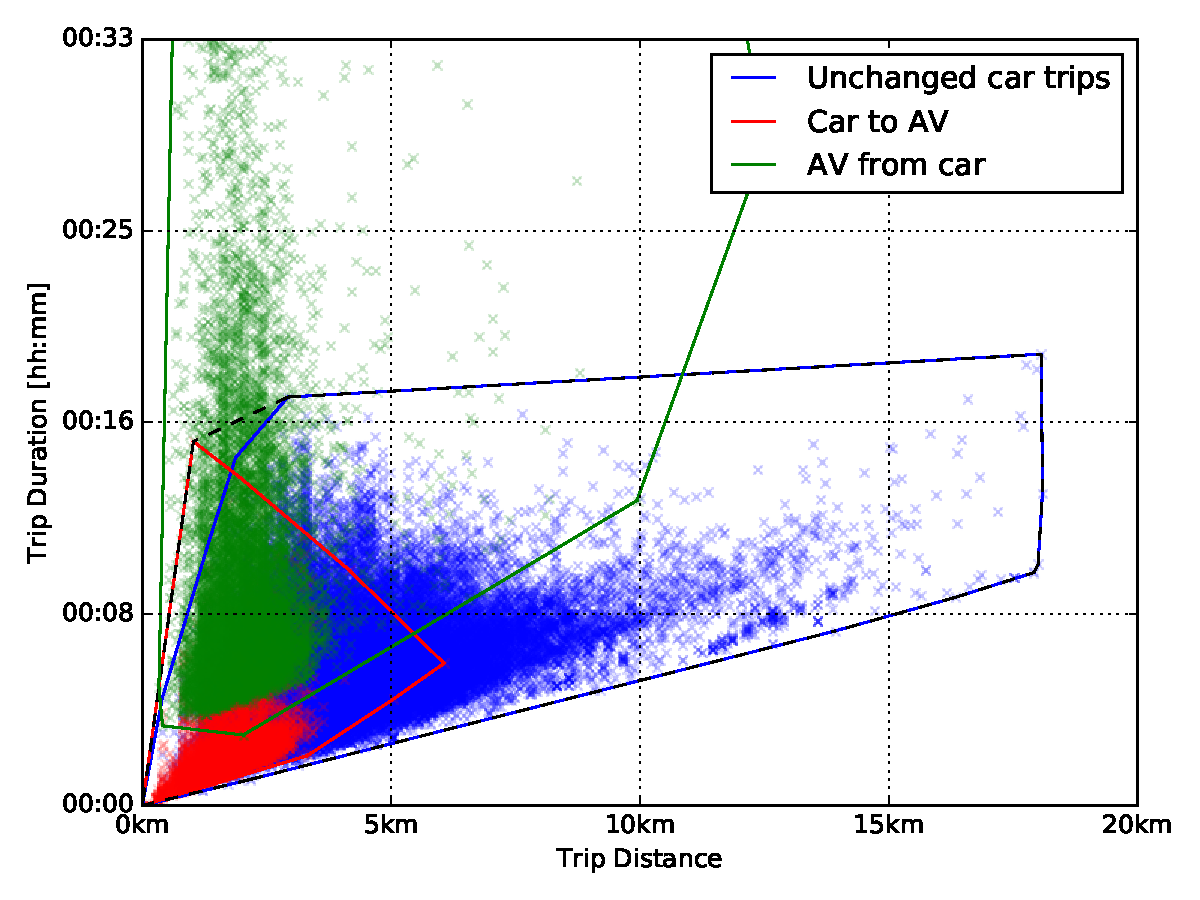
\includegraphics[width=0.9\textwidth]{figures/changes_car.pdf}
    \caption{Analysis of the distribution of public transport (top) and car (bottom) trips
    in terms of travel distance and duration before and after the introduction of
    autonomous vehicles.}
    \label{fig:changes_modes}
\end{figure}

\subsubsection{AV Operation and decreased supply}

Finally, \cref{fig:avwork} shows the states of the AVs during the day. While the
lines show how many AVs are currently performing either a pickup or dropoff task,
i.e. being ``en tour'', the shaded areas show how many passengers have been picked
up or dropped off at a certain time of the day. In this baseline scenario, only
around 3000 cars are actually active of the available 8000, so from the perspective
of an AV operator the scenario would not be an ideal case, because the
usage of the AVs is not nearly close to saturation.

\begin{figure}
    \centering
    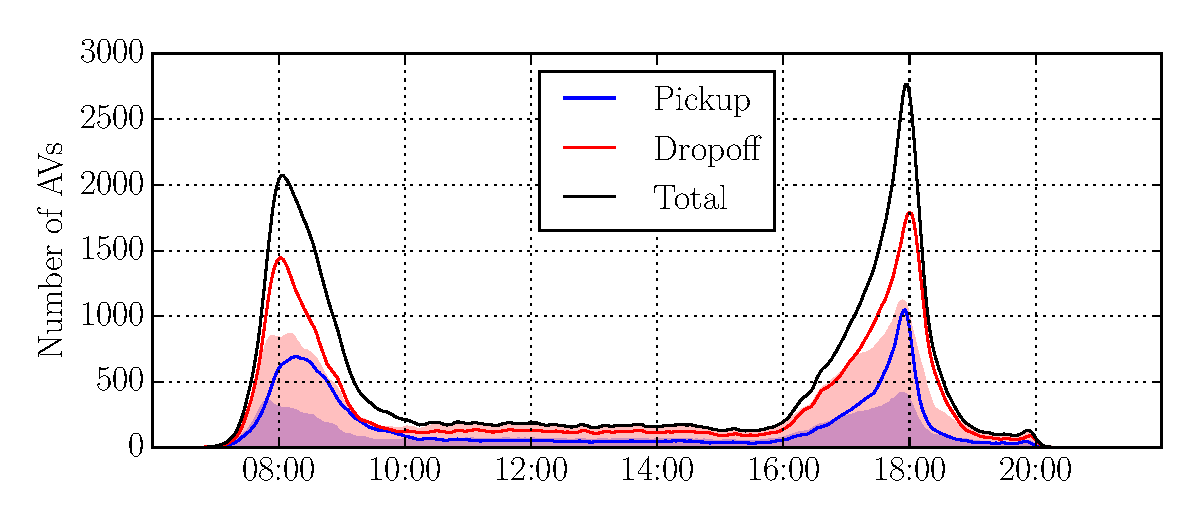
\includegraphics[width=0.9\textwidth]{figures/avwork.pdf}
    \caption{Activities of AVs during the day in the relaxed (8000 AVs) AV baseline scenario.
    The solid graphs show the number of vehicles, which are ``on tour'', while the
    shaded area denotes the number of pickup and dropoff interactions with the
    passenger.}
    \label{fig:avwork}
\end{figure}

Such a case is depicted in \cref{fig:avwork_low}. It shows the states of the AVs during the day
if only 1000 of them are available. Shaded areas
indicate those times of the day where the dispatchment mode changes from
oversupply to undersupply, where there are more requests than available AVs. At those
peak times, one
can see that the number of active AVs goes into saturation. The number does not
go to 1000 exactly since only driving AVs are measured, whereas some might be in
the 120s pickup or 60s dropoff activities.

\begin{figure}
    \centering
    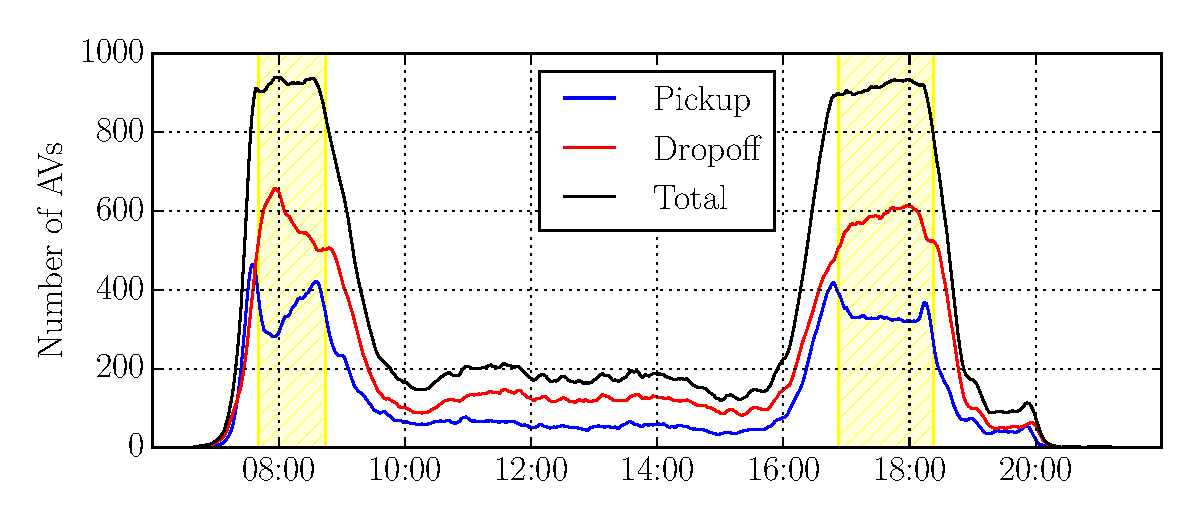
\includegraphics[width=0.9\textwidth]{figures/avwork_low.pdf}
    \caption{Activities of AVs during the day in the constrained (1000 AVs) AV baseline scenario.
    The show the number of vehicles, which are ``on tour'', while the
    shaded area denotes times where the undersupply dispatchment mode is active.}
    \label{fig:avwork_low}
\end{figure}

Compared to the high supply case, the share of AV trips drops from 25.19\% to
18.92\%. While the travel time stays roughly the same for the AV mode, the
average distance increases slightly from 2.94km to 3.18km, indicating a shortfall
of short trips. Around half the amount of private car users
switch to AVs (6.65\%, before 13.69\%); for public transport users, the decrease
is less significant from 44.29\% to 40.29\%. From that one can conclude that the
attractiveness of AVs for private car users is decreasing substantially with a
constrained supply while the induced longer waiting times seem to be tolerable
by former public transport users.

\begin{figure}
    \centering
    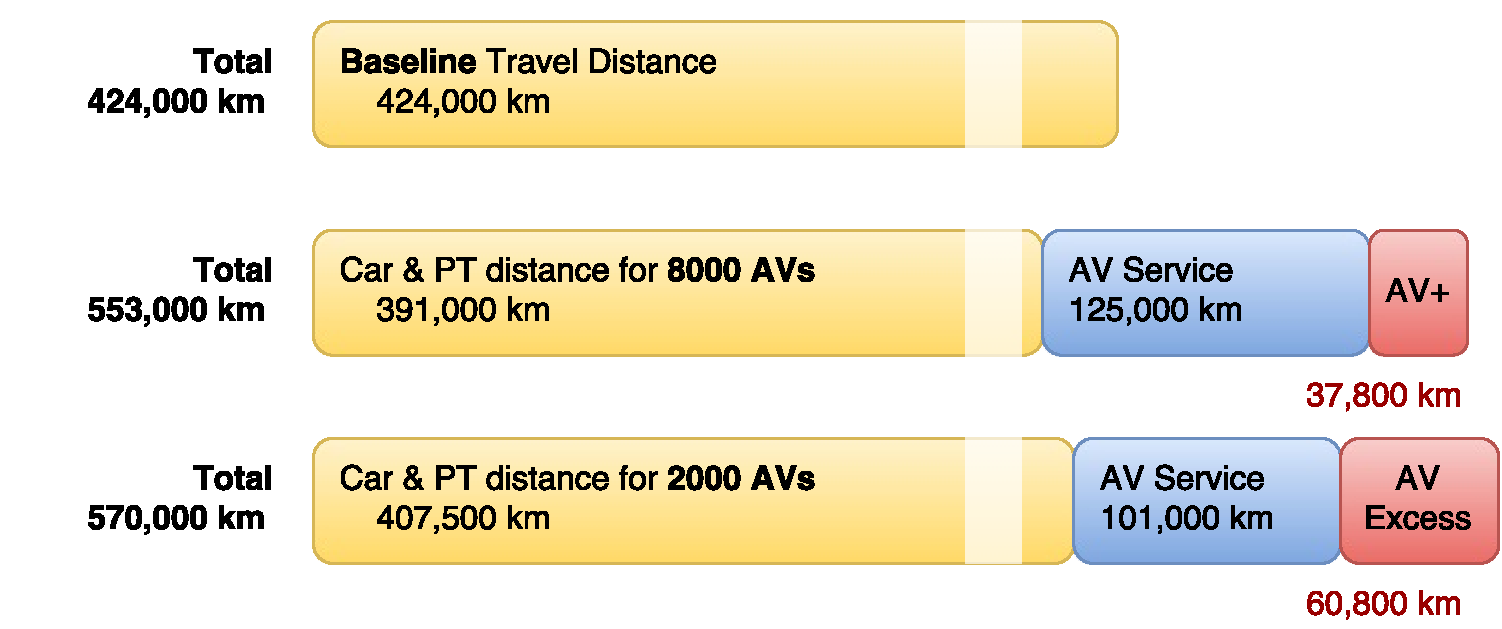
\includegraphics[width=1.0\textwidth]{figures/traveldistances.pdf}
    \caption{Comparison of total travel distances in the low and high supply scenarios.}
    \label{fig:traveldistances}
\end{figure}

From an environmental perspective, this scenario
is worse than the former one. While car users continue using their private vehicles,
public transport users switch to additional cars on the road. In terms of distance
(\cref{fig:traveldistances}), the total amount of kilometers driven increases further
because of an increase in excess travel distance of the AVs. Since fewer agents are
using the service, the vehicles have to cover longer distances to get to the next
customer. Such a case is disadvantageous for the service operator, so it will be
interesting to see how the additional costs of excess mileage affect the overall
economic evaluation of the provider (\cref{sec:economics}). The next chapter will
give a more detailed relation of the supply level on the total traveled distance.

\subsection{Supply Analysis}
\label{sec:waitingtimes}

\Cref{fig:excessdistance} shows the relation of travel distance and supply in
a more detailed way. At around 1000 vehicles, there is a peak of the net driven
distance in the network (black), which is relaxed if the supply is increased. The
stable added number of kilometers is then around 120,000km. However, the peak is
only 40,000km bigger than this value, which itself is a quarter of the initial
400,000km in the base scenario. Looking at the red graph, which shows the added
miles of empty drives in the AV services compared as an offset to the total number
of AV miles, one can see that it shows the same peak, i.e. the excess mileage is
responsible for the increase in total travel distance. In this regard, the service
operator and public administration would have the same priority to avoid this peak
(in terms of profit one one side and regarding environmental policy and congestion on the other).

\begin{figure}
    \centering
    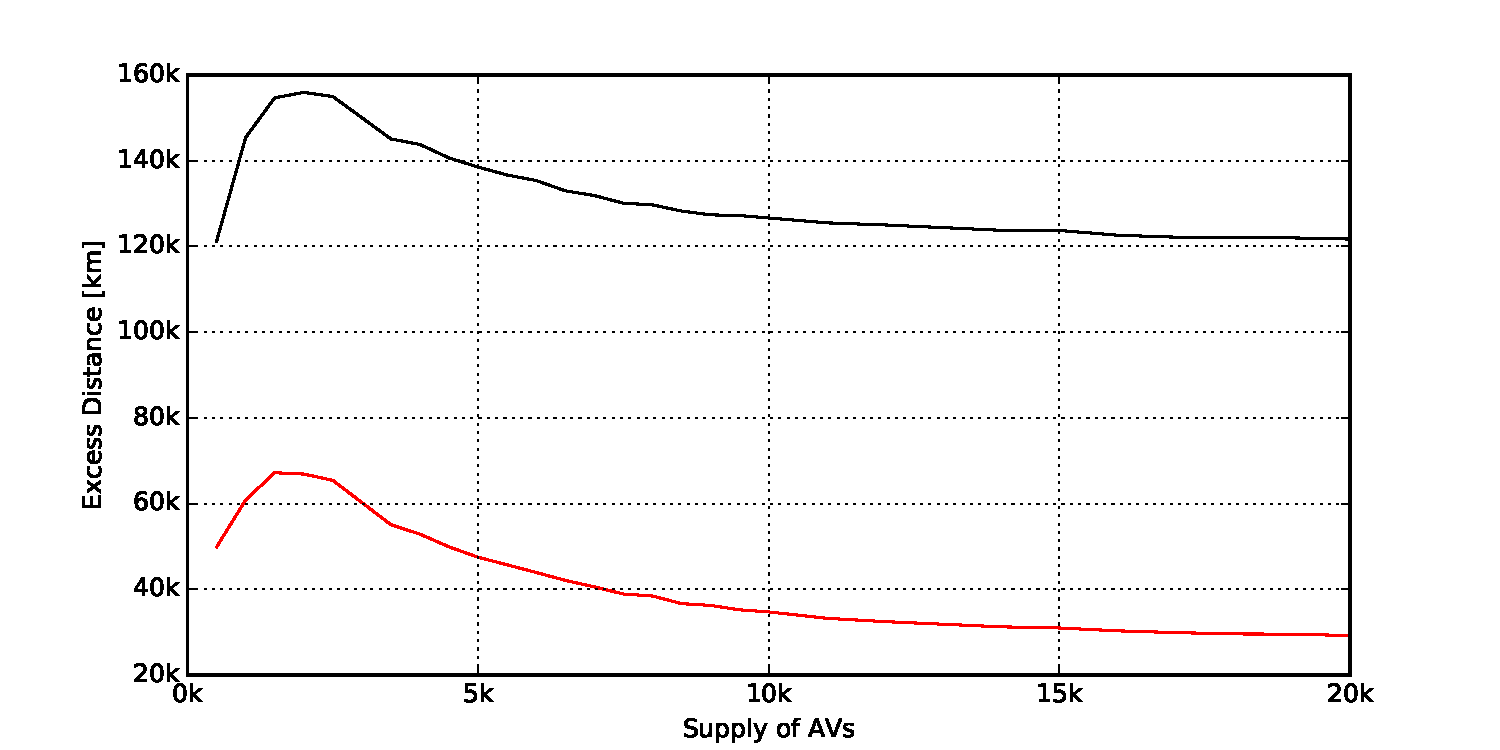
\includegraphics[width=0.9\textwidth]{figures/excessdistance.pdf}
    \caption{Evaluation of the total added travel distance of all vehicles compared
    to the base scenario without AVs (black) and excess driving distance for AVs
    for the respective supply (red).}
    \label{fig:excessdistance}
\end{figure}

In terms of waiting time it has been found that per 1000 AVs around 4\% of
initial car trips in the scenario could be replaced with static demand in \cref{sec:replacement}.
Looking at the waiting times on top in \cref{fig:waitingsupply}
one can see that the mean value as well as the 90\% quantile of the waiting time
$t_W$ is under the threshold of 10 minutes, which has been examined before. Furthermore, the middle of
\cref{fig:waitingsupply} shows $P(t_W \leq 10 min)$, i.e. the probability of having
a waiting time of less than 10 min in the simulated supply scenarios. While this
probability clearly decreases with small fleet sizes, it still stays rather high
at 90\%. That is the case, because due to high waiting times, fewer trips are being
made. For higher supplies, the quantile finds an equilibrium-like state at around
97\%, which can be interpreted as a measure of how tolerable increased waiting times are
in a certain scenario.

Additionally, the bottom plot in \cref{fig:waitingsupply} shows the replaced
percentage of trips dependent on the amount of available AVs. Because of the
preferences that are induced through the utility-based learning, considerably
fewer trips are converted to AVs although staying in the waiting time limits.
While in the static analysis 5000 AVs can replace 20\% of private car trips,
in the dynamic one it is only 15\%. For the static case 60\% are simulated
at 15,000 AVs, but here the replacement fraction remains at 15\%. This shows
that the usefulness of the mode, which is quantified by the utility, is the
restricting factor, despite a large available margin in waiting time efficiency.

\begin{figure}
    \centering
    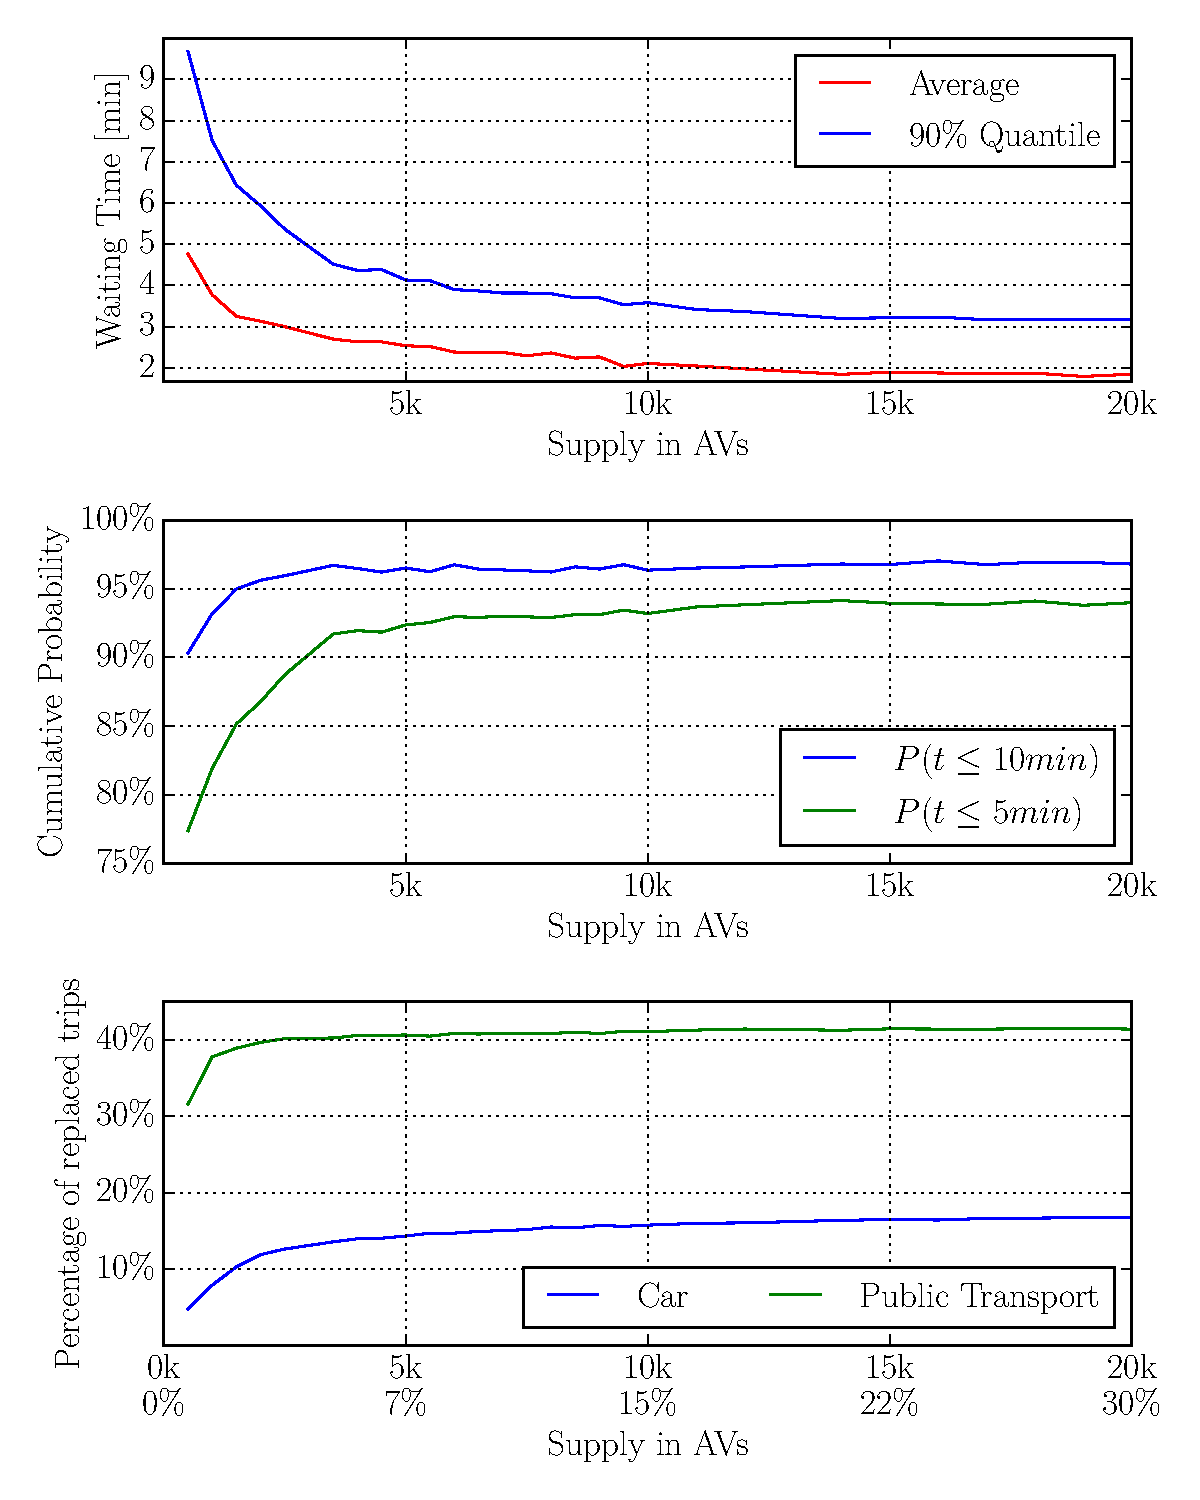
\includegraphics[width=0.9\textwidth]{figures/waitingsupply.pdf}
    \caption{Top: Mean value and 90\% quantile of waiting time for different supply
    levels. Bottom: Cumulative probability of observing a waiting time less than
    10 minutes.}
    \label{fig:waitingsupply}
\end{figure}

\subsection{Cost Dependencies}
\label{sec:costs}

Intuitively, the behavior of the utility parameters should be quite clear: If
the utility is increased, the AV mode gets more favorable, if it is decreased, less
people will use it. However, in such a complex traffic system there are secondary
effects, which influence the adaptation of AVs.

\Cref{fig:sharegrid} shows the share of the AV mode in the baseline scenario (top)
with different pricing schemes, given through a price per kilometer and a price
per trip. For near zero cost services, the share reaches 90\%, while for a combination
of \$7 per trip and \$3 per kilometer the share drops down to under 10\%. It can
be seen that for a very low travel utility (lower left) the threshold in the shares
gets steeper while it dilutes for  very high travel utility (i.e. acceptance)
of the AV mode (lower right). This hints at the fact that the more accepted AV
technology is in the population, the more people will use it while the pricing
scheme can have a huge impact on adaptation if there is a considerable amount of
skepticism towards the technology.

\begin{figure}
    \centering
    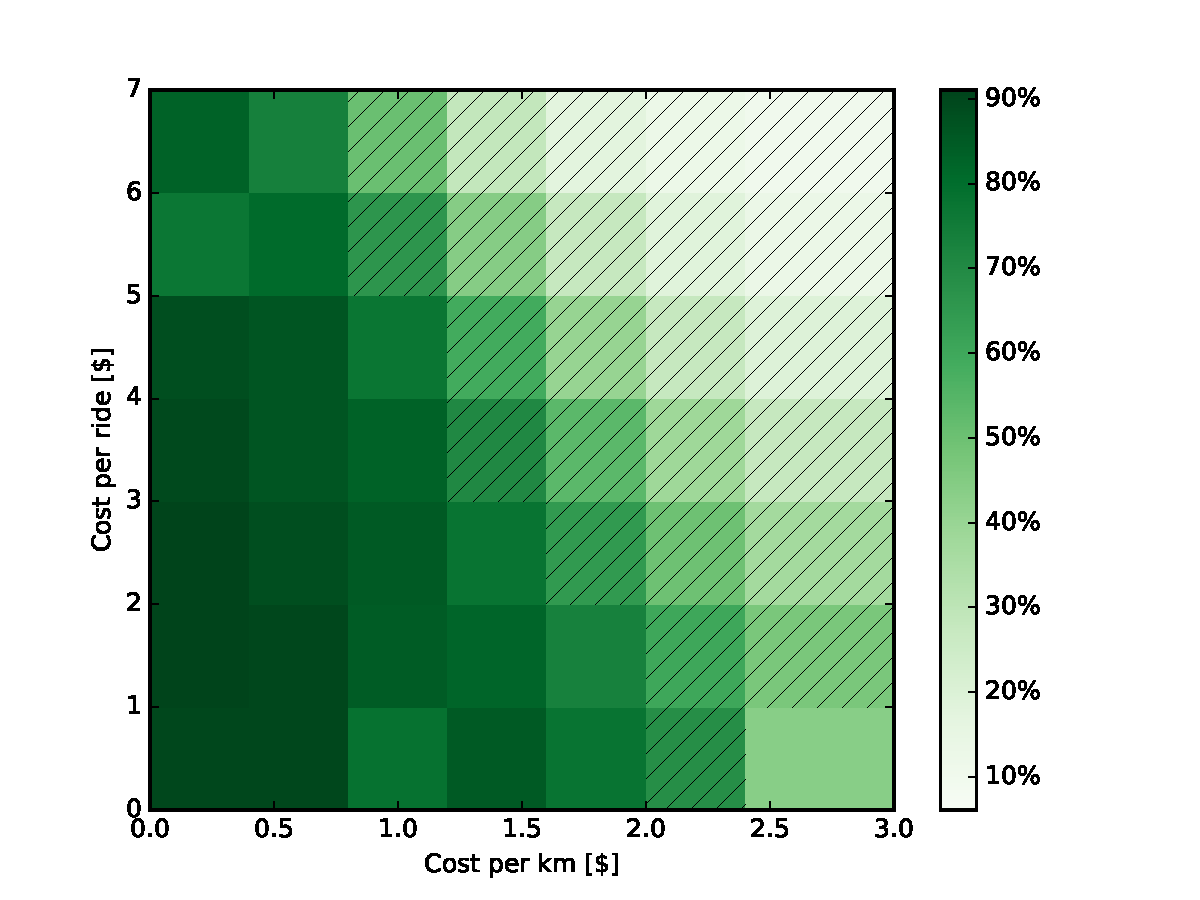
\includegraphics[width=0.9\textwidth]{figures/sharegrid.pdf}
    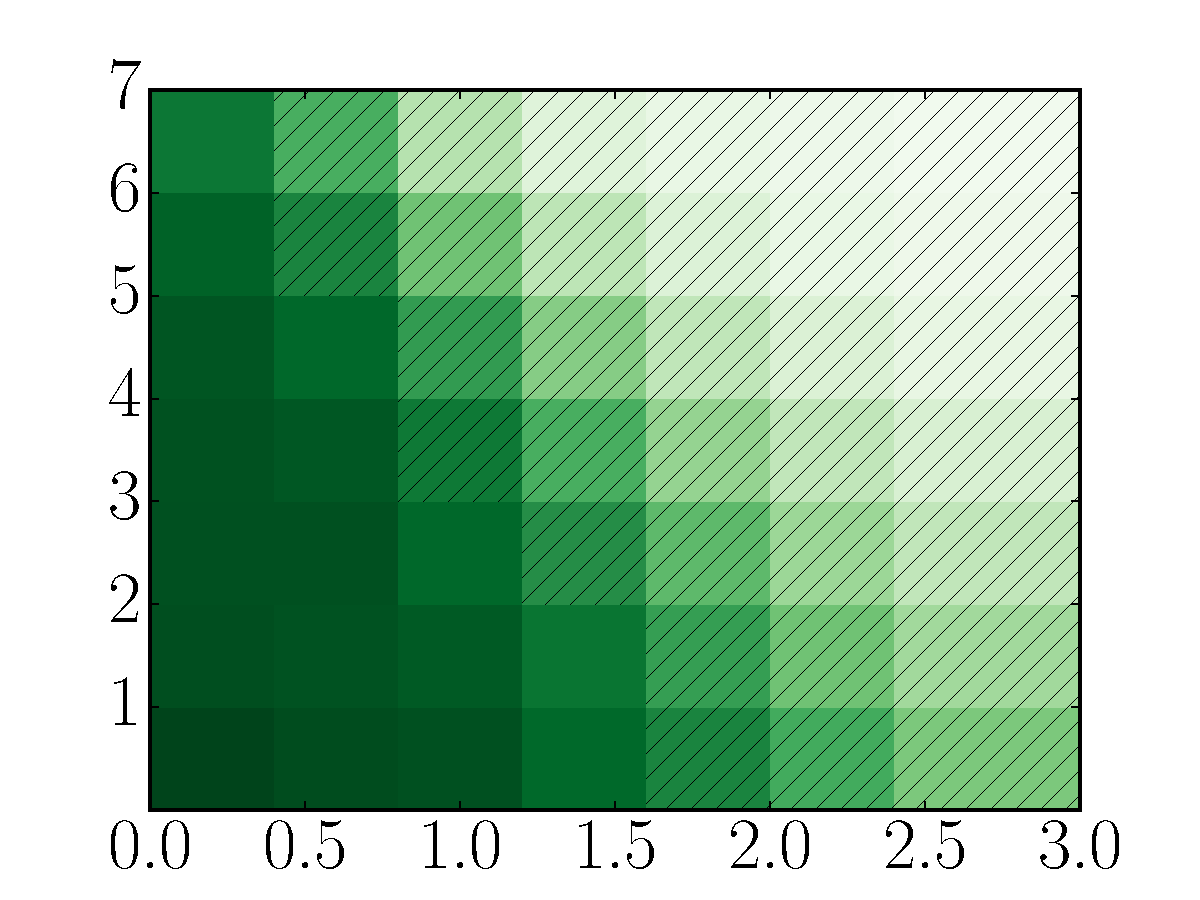
\includegraphics[width=0.45\textwidth]{figures/sharegrid_n05.pdf}
    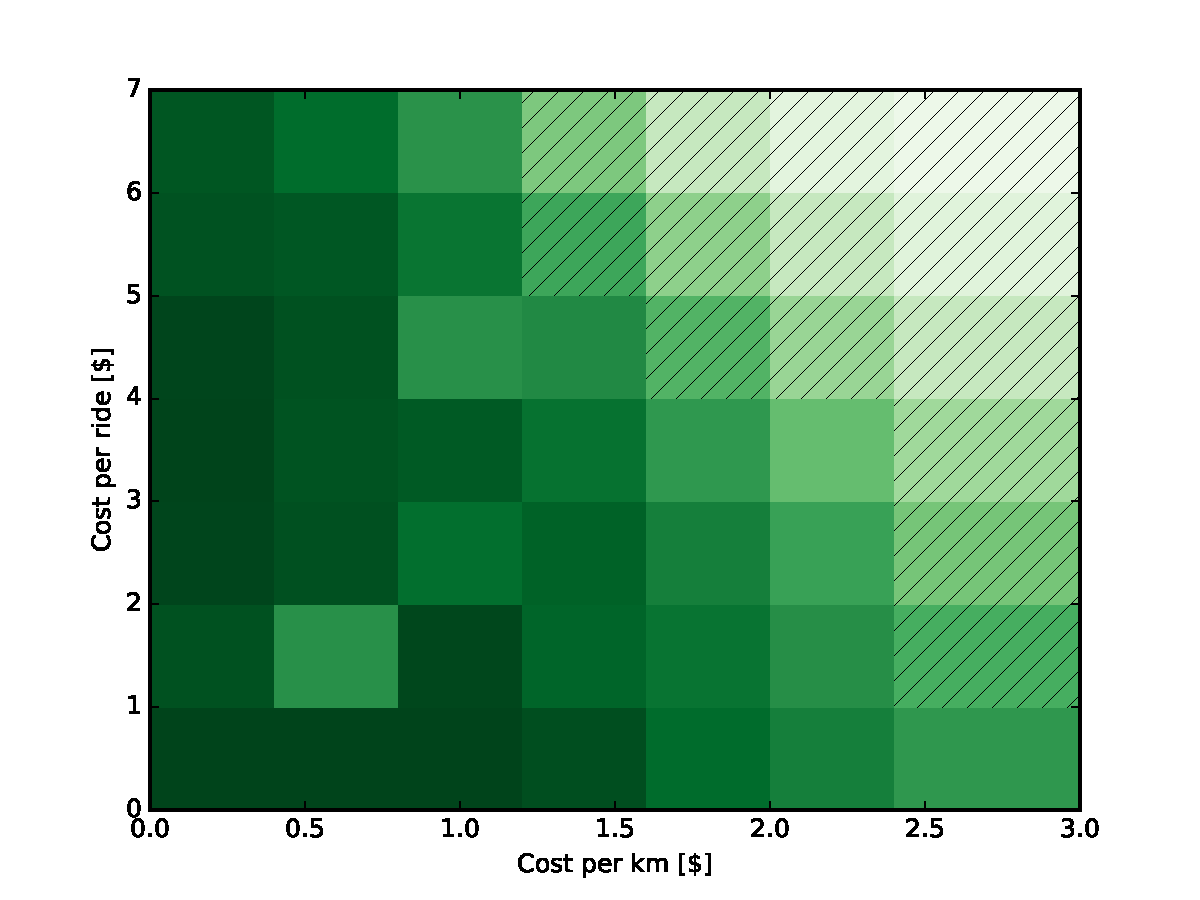
\includegraphics[width=0.45\textwidth]{figures/sharegrid_p05.pdf}
    \caption{Dependency of the AV mode share on the pricing scheme. Top: Baseline
    scenario. Left: Low utility of traveling ($\beta_{trav,av} = -0.5$). Right: High utility
    of traveling ($\beta_{trav,av} = 0.5$). Shaded areas show parameter combinations
    where the waiting time for an AV is shorter than 10 min in 90\% of the cases.}
    \label{fig:sharegrid}
\end{figure}

The shaded areas in \cref{fig:sharegrid} show those parameter combinations, where
$P(t_w \leq 10min) \geq 0.9$, i.e. where the probability to wait less than 10
minutes for an AV per trip is higher than 90\%. Taking that as another criterion
to assess the performance of an AV service, one can see that it puts a restriction
on how low the prices can drop to allow for a smooth operation of the
service. In fact, if waiting time is a constraint, only moderate shares of AVs
can be reached on any level of acceptance.

What needs to be kept in mind here is that no further investigations on the
disutility of waiting time have been performed here, but it is rather based on an
assumption taken from \citet{Chakirov2014}. Nonetheless, the result is surprising
since, in extreme cases, agents accept a waiting time of 30 minutes or more in
90\% of trips, as can be seen in \cref{fig:waitingtimegrid}. Mainly, this depends
on all the utility parameters in the scenario, also the utility of performing an
activity, the disutility of using other means of transport and so forth. Accepting
such a high waiting time might be an indicator that the utilities in the Sioux
scenario should be further improved to lead to better results. However, the interpretation
is tricky for very low prices, since they also resemble quite unrealistic situations, where
only times are weighed against each other: If there are no monetary costs, a trip
in terms of utility costs as much as not performing an activity for the travel time.

Furthermore, the results of the simulation are surprising when looking at the share
of public transport in \cref{fig:ptsharegrid}. The general tendency makes
sense: Lower prices lead to lower shares of public transport because using an AV
gets more advantageous. Also, having very high prices, the public transport share
stays at its initial baseline level. Nevertheless, one would expect people to
react more abrupt to the pricing scheme on the per-trip side than on the per-km
side. So far each trip in the Sioux Falls scenario costs \$2. Imposing no per-trip
fee for AVs, but different per-km fares should show a smooth transition as can be seen
in \cref{fig:ptsharegrid}: The shares
should change depending on the price and the trip distance distribution.
On the other hand, if no per-km fare is imposed, but only per-trip payments, the
transition should be more abrupt. This effect, however, might be smoothed out by
AVs taking less travel time.

This is only true though if people can make rational decisions about the
total costs of travel. When looking at the beforementioned plots, one can see
that there is are quite linear nivau lines, meaning that if a per-km cost is given,
one can easily obtain the per-trip cost in order to stay at a certain level of
service. For instance, this means that for the agents, paying \$5 per trip and
\$1.60 per km is equal to paying \$3 per trip and \$1.90 per distance. In reality, the perception of the high per-trip fare might be different to the lower
per-km fare, especially compared to the initial \$2 per trip.

\begin{figure}
    \centering
    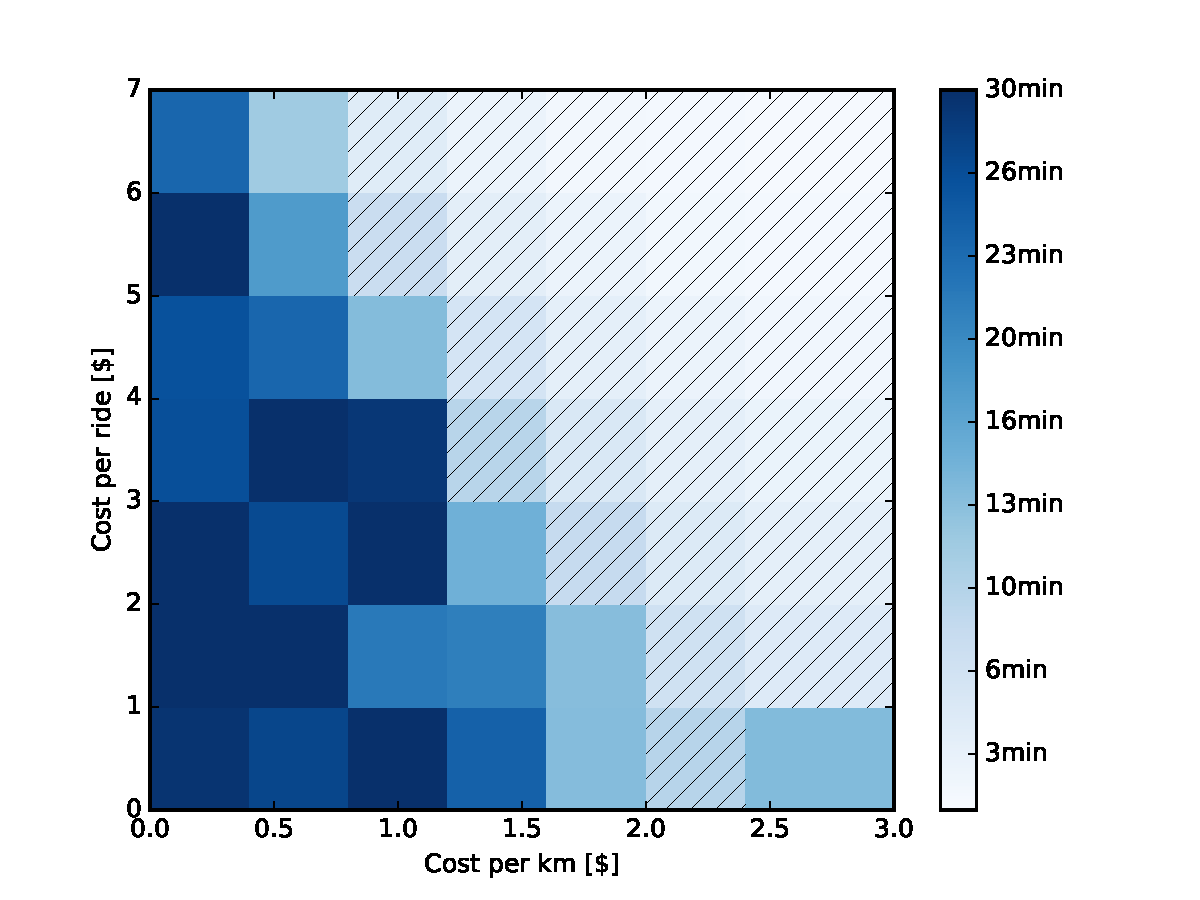
\includegraphics[width=0.85\textwidth]{figures/waitingtimegrid.pdf}
    \caption{90\% quantile of the waiting time in the baseline scenario with different
    pricing schemes. The scale is truncated at 30 minutes.}
    \label{fig:waitingtimegrid}
\end{figure}

\begin{figure}
    \centering
    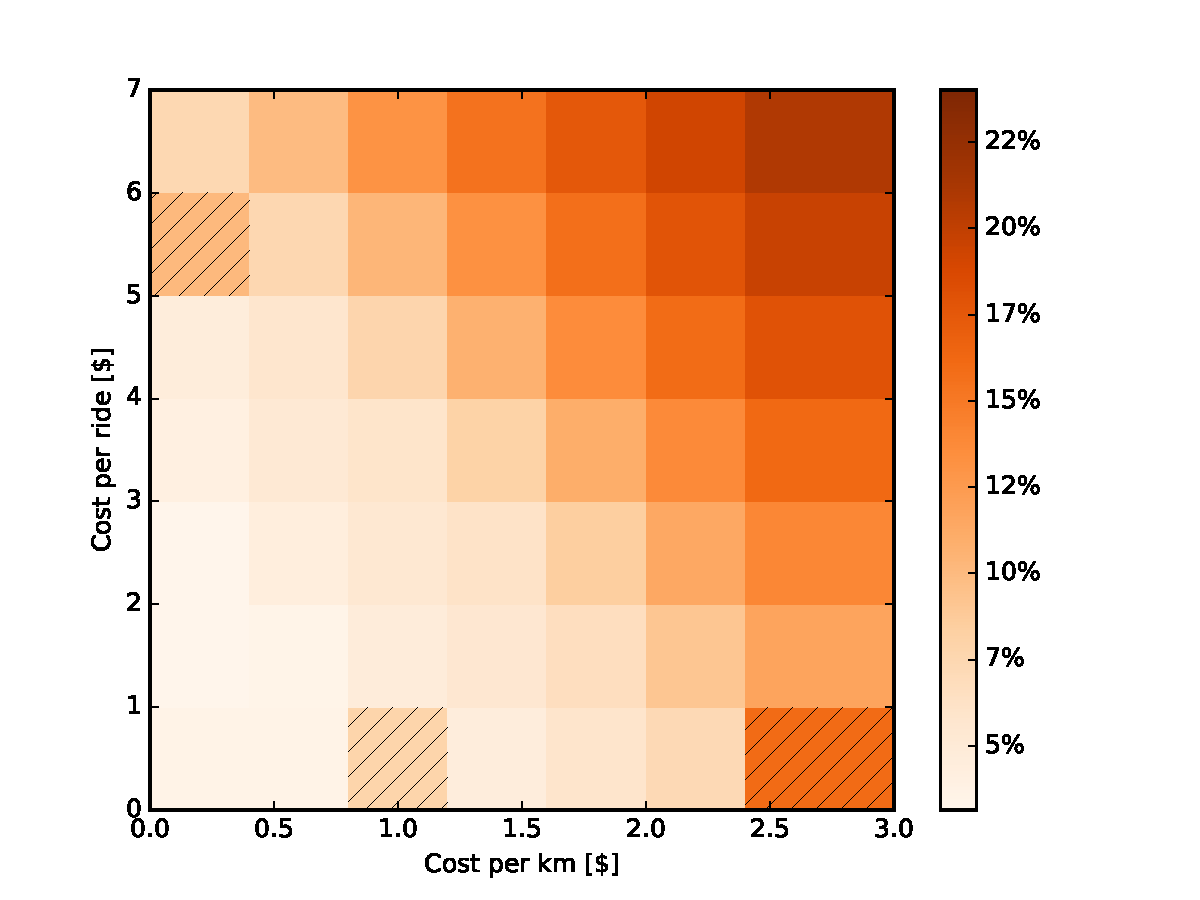
\includegraphics[width=0.85\textwidth]{figures/ptsharegrid.pdf}
    \caption{Share of public transport
    trips. Shaded areas indicate not completely relaxed simulation runs with stuck agents.}
    \label{fig:ptsharegrid}
\end{figure}

Combining the results of this section, it becomes apprent that in the given scenario,
also the share of public transport has a lower bound if a specific service level in
terms of waiting time should be maintained. On the other hand, the introduction of
AV services will diminish the share of public transport in any case. As one conclusion
it can be therefore stated that without any policy-based incentives, it is not possible
to maintain the level of public transport while motivating private car owners to switch to AVs.

Another point that has to be taken into account regarding these considerations is
the profitability of the service for the operator, which will be the subject of the
next section.

\subsection{Economic Analysis}
\label{sec:economics}

The operator model for the net income $z$ proposed in this thesis can be stated as follows:

\begin{equation}\begin{aligned}
z
&= \underbrace{p_{km} \cdot d_{dropoff} + p_{trip} \cdot n_{trips}}_{Gross Income}\\
&- \left( \underbrace{\$6 \cdot n_{veh} + c_{pd} \cdot n_{veh} + \gamma_{d,car} \cdot d_{total}}_{Expenses} \right)
\label{eq:step1}
\end{aligned}\end{equation}

On the income side of the operator, there is the total distance of dropoff (i.e.
occupied) trips $d_{dropoff}$, multiplied by the price per km and the number
of AV trips $n_{trips}$, multiplied by the price per trip. The expense side has
been modeled to be comparable with the car mode in the Sioux-16 scenario. It involves
a cost for parking (\$6) as well as running costs per km for private cars multiplied by the combined
total distance for pickup and dropoff trips. Of course, this choice bears a lot
of uncertainty, it might be a reasonable guess though, since increased costs for
insurance and decreased costs for (electric) operational costs might weigh out
each other \citep{Chen15}. Finally, a cost per day
$c_{pd}$ is introduced for each supplied AV taxi.

That cost has been modeled as follows: \Citet{Chen15} states predictions of
(electric) AV taxi prices of around $c_{veh} = \$62,000$ (converted to AUD) and states lifetimes
of around $d_{max} = 370,000 km$. From the simulation the average driven distance
of one day is known as $d_{avg} = d_{total} / n_{veh}$ per vehicle. Those values can
be used to obtain a vehicle lifetime, assuming that the amount of kilometers
driven stays constant over the lifetime $\tau$:

\begin{equation}
\tau = \frac{d_{avg}}{d_{total} / 1d} = \left[ \frac{km}{km/d} \right] = [d]
\end{equation}

Then the costs per vehicle per day can be stated as:

\begin{equation}\begin{aligned}
c_{pd} &= \frac{c_{veh}}{\tau} = d_{avg} \cdot \frac{c_{veh}}{d_{max}} \\
&= d_{avg} \cdot \nu\\
&= \nu \cdot \frac{d_{total}}{n_{veh}}
\end{aligned}\end{equation}

with

\begin{equation}
\nu = 0.17 \frac{\$}{km}.
\end{equation}

Inserting this equation into \cref{eq:step1} effectively cancels out the number
of available AVs from the investment costs and integrates them into the per
distance costs:

\begin{equation}\begin{aligned}
z
&= \underbrace{p_{km} \cdot d_{dropoff} + p_{trip} \cdot n_{trips}}_{Gross Income}\\
&- \left( \underbrace{\$6 \cdot n_{veh} + (\nu + \gamma_{d,car}) \cdot d_{total}}_{Expenses} \right)
\label{eq:step1}
\end{aligned}\end{equation}

Therefore the net income is characterized by a complex relation of the total distance
driven, the occupied distance, the number of cars and the number of AV trips. Applying
this model to the previously introduced pricing scheme map gives the result in
\cref{fig:netincomegrid}. For very low prices the service clearly is not profitable
in the proposed model, while it is possible to maintain the service in a moderate
price range. In fact, the area with most profit is covered by the formerly introduced
condition on waiting times (hatched area). However, from an administrative perspective,
one might also want to maintain a certain share of public transport. Here, a arbitrary
share of 15\% is chosen, which should be maintained. In that case the operator would need to offer the service
in the crossed area. There the profit is decreasing because of a smaller
number of users.

For the baseline scenario, the operator scenario has been tested with different
supply levels. The results in \cref{fig:revenuesupply} show that over the whole
range of AVs there the service is profitable, especially at 4000 AVs. Over the whole
depicted range the constraints on waiting time and public transport are fulfilled.
In that sense those scenarios are quite optimal cases, where the share of
public transport stays above 15\%, the waiting times are usually less than 10
minutes and the operator has a large margin. Incorporating the results from
\cref{sec:baselinesc}, the right-most cases are the best because additionally
the overall excess mileage is smallest.

The large margin is an indicator that the baseline scenario is a setup
that could ``work'' in a city similar to the Sioux Falls network. Contrary to
the financial analysis in \Citet{Chen15}, here infrastructure costs have not been
included in the analysis, which could be covered by that profit of the operator.

\begin{figure}
    \centering
    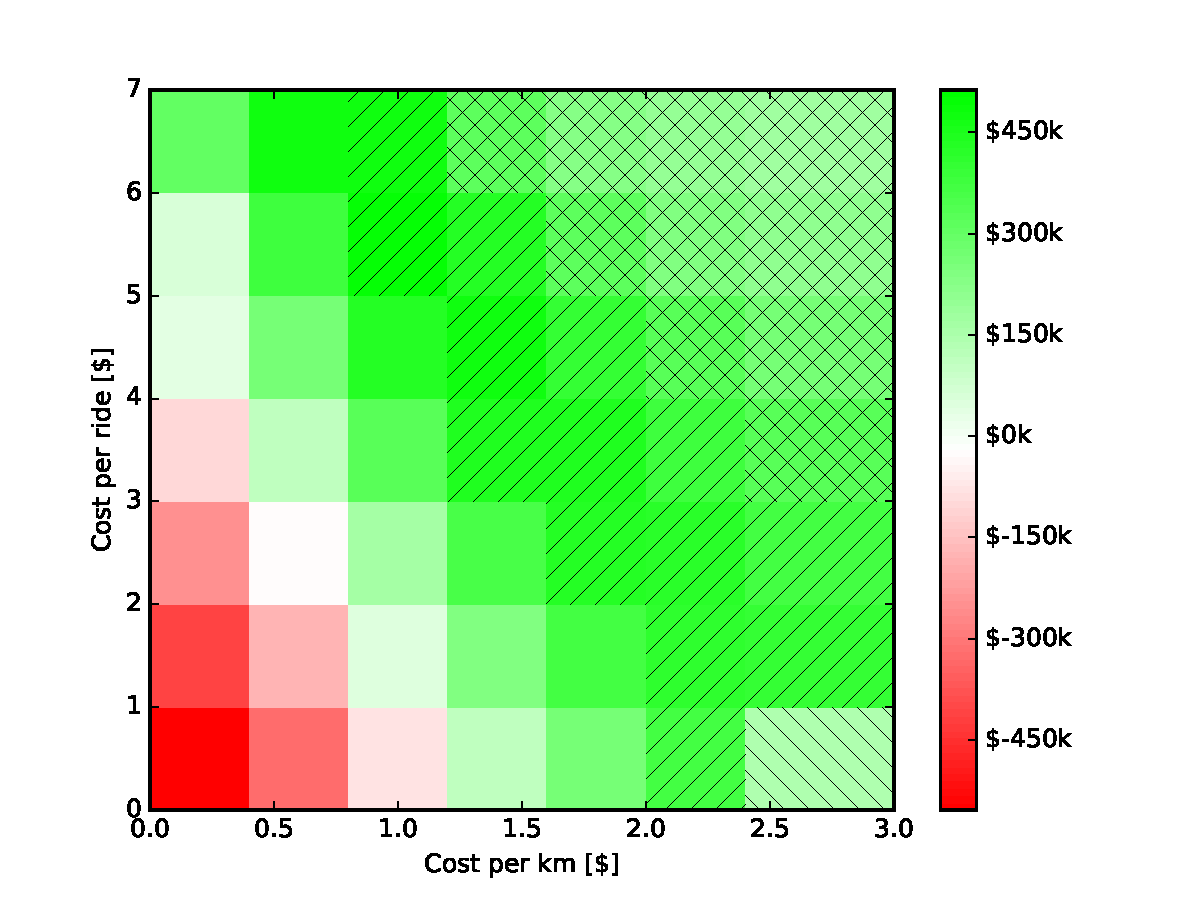
\includegraphics[width=0.9\textwidth]{figures/netincomegrid.pdf}
    \caption{Net income of the AV operator. The shaded areas represent acceptable
    waiting times (bigger area) and public transport mode shares of more than
    15\% (smaller area).}
    \label{fig:netincomegrid}
\end{figure}

\begin{figure}
    \centering
    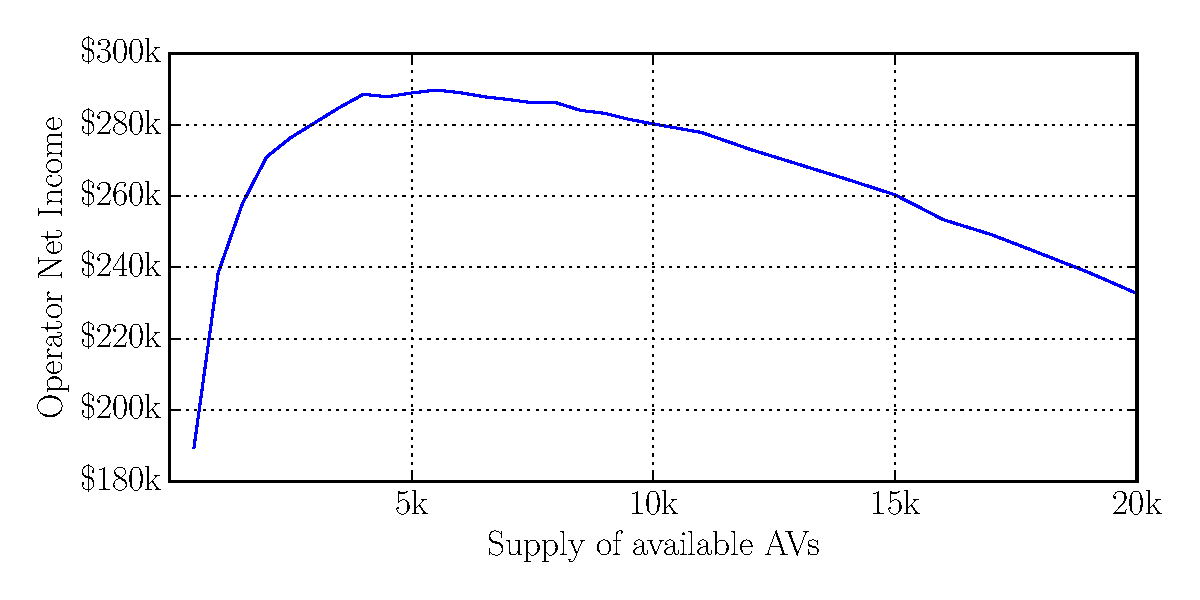
\includegraphics[width=0.9\textwidth]{figures/revenuesupply.pdf}
    \caption{Dependency of the operator net income in the baseline scenario on
    the number of supplied AVs.}
    \label{fig:revenuesupply}
\end{figure}
 \FloatBarrier \pagebreak
\section{Outlook}
\label{sec:outlook}

During the course of this thesis a versatile and extentable basis model for the
simulation of autonomous vehicles has been developed. Many topics in the field
which would be interesting to investigate were not part of the scope of this thesis.
The following sections will present the most important and interesting ones and
give directions on how to simulate them with the framework. Likewise, these sections
also give an overview about critical points, which are not taken into account in
the previous results, but could change the overall picture significantly.

Four different aspects will be put into focus:

\begin{itemize}
\item Extensions of the infrastructure
in the model, which would account for what needs to be done to maintain the AV
service in a more realistic and/or efficient way,
\item the interaction with the AV service, widening the possibilities that one
or multiple agents have to take advantage of the new travel mode, and
\item extensions to the current demand simulation.
\end{itemize}

\subsection{Infrastructure Extensions}

Since autonomous vehicles in general will take great advantage of the ongoing
electrification in the automotive industry, the availability of the respective
infrastructure is one factor which can determine how fast the adaptation of AVs
will progress \citep{Burmeister2016}.
Given the right amount of resources to create such an infrastructure, a big question
that arises is how many recharging facilities are needed and where they should begin
located in order to serve certain sizes of AV fleets \citep{Chen2015}. Furthermore, how can a combined
infrastructure for ordinary owned EVs, private AVs and publicly provided AV services
be designed?

As a first step one could assume that AVs recharge at dropoff locations, where they
are artificially put to rest for a certain minimum idle time in order to simulate
the recharging process. This would already lead to results on the customer acceptance
side, but would ignore effects on congestion if AVs would actually need to take long
trips to the next charging facility. Previous studies using MATSim already gave interesting results on the implementation
of eletrified taxis in Berlin with distributed charging facilities
over the network \citep{Bischoff2014}. Such research could be combined with the AV framework developed here.
The modular AgentFSM component would make it easy to add specific new points in the
state chains of an AV to drive to a charging facility. Then again, the simulation framework could be used to get insights in which scheduling
strategies would be optimal for an AV fleet if recharging has to be taken into account.

Another idea to improve the simulation is to introduce means of simulating maintenance
and parking. So far it has been assumed that autonomous vehicles will reside where the last
dropoff has taken place. This assumption, especially in heavily packed cities, is
quite optimistic, since parking space might be rare. In consequence, the driven
kilometers per AV in the unoccupied state could be quite off the actual distance.
More mileage would be needed to find a parking space in between tasks.
This rises a whole range of questions on how an optimal AV scheduling would
look like, maybe depending on the demand level, it might be even interesting to
run  studies on whether the search for parking space might be inferior
to roaming around.

This could be done in combination with intelligent repositioning, where in between peak
hours taxis could be intelligently moved to likely pickup positions and thus minimize the waiting
time for customers, increasing the acceptance and reducing
operator costs at the same time because less unoccupied miles might be travelled.

With the parallelization of customer trips the presented framework already shows
by example how such an algorithm could be incorporated into the existing infrastructure
without having too much impact on the computation times. In general, doing ``some''
intelligent repositioning should always be more beneficial than doing none. In
this regard, the repositioning could be computed in parallel to the ongoing
traffic simulation, while still offering the ability to restrict it if it slows
down the main loop of MATSim.

\subsection{Usage and interaction with the AV service}

The AV service in the developed model so far is very basic in the way customers
are able to interact with it. One obvious advantage of AV fleets is, that up to five people could be transported
in ordinarily shaped cars and even more in autonomous minibusses or full-sized busses.
Intelligent routing and scheduling algorithms would make it possible to pick up passengers
at arbitrary locations, not being bound to a fixed public transport schedule.

Due to the extensible structrue of the AV extension, it would be easy to
add such behaviour in principle. However, the problem of optimizing the trips of
more than one passenger, probably while already on a ride, is a highly complex
problem and acceptable heuristics are still an important research subject.
Adding such functionality to the AV framework would make it possible to test such
strategies in near-realistic scenarios and measure the performance of different
heuristics.

Additionally, autonomous vehicles are likely to relax the last mile problem, where people are not
motivated to opt for public transport, because the last mile from the transport
facility to their home is too long. An AV could bridge this distance, maybe being
prescheduled to pick up the passenger according to the current expected arrival
times.

Implementing this behaviour would need only small changes in the MATSim framework.
Generally, a public transport trip is generated as three legs: One \texttt{transit\_walk}
leg in order to get to the stop facility, one \texttt{pt} leg for the actual residual
time in the bus  and another \texttt{transit\_walk}. A first attempt
would be to replace some of the \texttt{transit\_walk} legs during the planning
phase with \texttt{av} trips, which could already lead to a convincing simulation
of AVs feeding the public transport network.
A probable requirement for this to work well would be to have prescheduled AVs
to give a higher reliability on these connections.

Prescheduled autonomous vehicles would be easy to implement in the existing infrastructure.
In fact, test have already been done, but abandoned due to the fact that in a first
approximation delays from the scheduling can be modeled using worse utility values
for the waiting times.
In the current state, the AV framework fully supports such prescheduled trips, though
their impact has not been investigated in the scope of this thesis. As shown in
figure \cref{fig:avstates}, where the state diagram of the AV is depicted, a ``Waiting''
state is already included, which would make an AV which arrives early at a pickup
location wait for the passenger.

\subsection{Demand Analysis}

An intereting point in the simulation is the spatial dependence. On one side,
it would be interesting to investigate where AV users live, maybe indicating that
on specific pricing strategies, people from the suburbs prefer AVs, while other
strategies might encourage people living in the center to use them.

Heavily related to that is the initial distribution of AVs at the beginning
of the daily simulation. As described before, AVs are currently distributed dependent on
the population density, though that might not be the best approach. Especially
if one wants to encourage suburbians to use AVs, the density there should be higher.

In that regard it would be beneficial to investigate how the initial conditions
in the MATSim simulation influence the result on an abstract level. For the case of
AVs, having initial AV plans mainly assigned to agents from a city center, but not for people
from the suburbs, the relaxed state might settle down in exactly this condition.
However, if AVs are mainly distributed in the suburbs in the initial plans, the
main user group might stay there, just because during the simulations the waiting
times are shorter in either case and therefore these people might stick to their
initial plan decisions. Therefore, a thorough investigation of the distribution
behavior of the algorithm would be very interesting.

Furthermore, the research in this thesis has shown that without any incentives, AVs might lead
to adverse effects, which should be corrected by intelligent policy decisions. \Citet{Chen16} suggests
interesting approaches of incentivizing AV usage. In order to ``free'' the city center
from too much congestion one could for instance in the Sioux Falls scenario put high monetary fees on using the streets within the
highway belt for private cars, while in parallel increasing the likelihood for AVs
to use the highways. This way one could try to move traffic to the highways, then
taking a direct trip to the workplaces in a perpendicular way.

Experiments like these are ready to be done with the existing simulation framework
by adding custom scoring functions for private cars and autonomous vehicles.

Finally, efforts have been made recently to diversify the population in MATSim simulations \citep{Chakirov2015}.
This means that people might be constrained or inclined due to age or income to use certain means
of transport. Combining the simulation of AVs with the introduction of that heterogeneity
could give insights on how the availability and pricing of AVs affect the distribution
of users in terms of a richer set of social variables.
 \FloatBarrier \pagebreak

\bibliography{references}

\end{document}
